% Options for packages loaded elsewhere
\PassOptionsToPackage{unicode}{hyperref}
\PassOptionsToPackage{hyphens}{url}
\PassOptionsToPackage{dvipsnames,svgnames,x11names}{xcolor}
%
\documentclass[
  letterpaper,
  DIV=11,
  numbers=noendperiod]{scrartcl}

\usepackage{amsmath,amssymb}
\usepackage{lmodern}
\usepackage{iftex}
\ifPDFTeX
  \usepackage[T1]{fontenc}
  \usepackage[utf8]{inputenc}
  \usepackage{textcomp} % provide euro and other symbols
\else % if luatex or xetex
  \usepackage{unicode-math}
  \defaultfontfeatures{Scale=MatchLowercase}
  \defaultfontfeatures[\rmfamily]{Ligatures=TeX,Scale=1}
\fi
% Use upquote if available, for straight quotes in verbatim environments
\IfFileExists{upquote.sty}{\usepackage{upquote}}{}
\IfFileExists{microtype.sty}{% use microtype if available
  \usepackage[]{microtype}
  \UseMicrotypeSet[protrusion]{basicmath} % disable protrusion for tt fonts
}{}
\makeatletter
\@ifundefined{KOMAClassName}{% if non-KOMA class
  \IfFileExists{parskip.sty}{%
    \usepackage{parskip}
  }{% else
    \setlength{\parindent}{0pt}
    \setlength{\parskip}{6pt plus 2pt minus 1pt}}
}{% if KOMA class
  \KOMAoptions{parskip=half}}
\makeatother
\usepackage{xcolor}
\setlength{\emergencystretch}{3em} % prevent overfull lines
\setcounter{secnumdepth}{-\maxdimen} % remove section numbering
% Make \paragraph and \subparagraph free-standing
\ifx\paragraph\undefined\else
  \let\oldparagraph\paragraph
  \renewcommand{\paragraph}[1]{\oldparagraph{#1}\mbox{}}
\fi
\ifx\subparagraph\undefined\else
  \let\oldsubparagraph\subparagraph
  \renewcommand{\subparagraph}[1]{\oldsubparagraph{#1}\mbox{}}
\fi

\usepackage{color}
\usepackage{fancyvrb}
\newcommand{\VerbBar}{|}
\newcommand{\VERB}{\Verb[commandchars=\\\{\}]}
\DefineVerbatimEnvironment{Highlighting}{Verbatim}{commandchars=\\\{\}}
% Add ',fontsize=\small' for more characters per line
\usepackage{framed}
\definecolor{shadecolor}{RGB}{241,243,245}
\newenvironment{Shaded}{\begin{snugshade}}{\end{snugshade}}
\newcommand{\AlertTok}[1]{\textcolor[rgb]{0.68,0.00,0.00}{#1}}
\newcommand{\AnnotationTok}[1]{\textcolor[rgb]{0.37,0.37,0.37}{#1}}
\newcommand{\AttributeTok}[1]{\textcolor[rgb]{0.40,0.45,0.13}{#1}}
\newcommand{\BaseNTok}[1]{\textcolor[rgb]{0.68,0.00,0.00}{#1}}
\newcommand{\BuiltInTok}[1]{\textcolor[rgb]{0.00,0.23,0.31}{#1}}
\newcommand{\CharTok}[1]{\textcolor[rgb]{0.13,0.47,0.30}{#1}}
\newcommand{\CommentTok}[1]{\textcolor[rgb]{0.37,0.37,0.37}{#1}}
\newcommand{\CommentVarTok}[1]{\textcolor[rgb]{0.37,0.37,0.37}{\textit{#1}}}
\newcommand{\ConstantTok}[1]{\textcolor[rgb]{0.56,0.35,0.01}{#1}}
\newcommand{\ControlFlowTok}[1]{\textcolor[rgb]{0.00,0.23,0.31}{#1}}
\newcommand{\DataTypeTok}[1]{\textcolor[rgb]{0.68,0.00,0.00}{#1}}
\newcommand{\DecValTok}[1]{\textcolor[rgb]{0.68,0.00,0.00}{#1}}
\newcommand{\DocumentationTok}[1]{\textcolor[rgb]{0.37,0.37,0.37}{\textit{#1}}}
\newcommand{\ErrorTok}[1]{\textcolor[rgb]{0.68,0.00,0.00}{#1}}
\newcommand{\ExtensionTok}[1]{\textcolor[rgb]{0.00,0.23,0.31}{#1}}
\newcommand{\FloatTok}[1]{\textcolor[rgb]{0.68,0.00,0.00}{#1}}
\newcommand{\FunctionTok}[1]{\textcolor[rgb]{0.28,0.35,0.67}{#1}}
\newcommand{\ImportTok}[1]{\textcolor[rgb]{0.00,0.46,0.62}{#1}}
\newcommand{\InformationTok}[1]{\textcolor[rgb]{0.37,0.37,0.37}{#1}}
\newcommand{\KeywordTok}[1]{\textcolor[rgb]{0.00,0.23,0.31}{#1}}
\newcommand{\NormalTok}[1]{\textcolor[rgb]{0.00,0.23,0.31}{#1}}
\newcommand{\OperatorTok}[1]{\textcolor[rgb]{0.37,0.37,0.37}{#1}}
\newcommand{\OtherTok}[1]{\textcolor[rgb]{0.00,0.23,0.31}{#1}}
\newcommand{\PreprocessorTok}[1]{\textcolor[rgb]{0.68,0.00,0.00}{#1}}
\newcommand{\RegionMarkerTok}[1]{\textcolor[rgb]{0.00,0.23,0.31}{#1}}
\newcommand{\SpecialCharTok}[1]{\textcolor[rgb]{0.37,0.37,0.37}{#1}}
\newcommand{\SpecialStringTok}[1]{\textcolor[rgb]{0.13,0.47,0.30}{#1}}
\newcommand{\StringTok}[1]{\textcolor[rgb]{0.13,0.47,0.30}{#1}}
\newcommand{\VariableTok}[1]{\textcolor[rgb]{0.07,0.07,0.07}{#1}}
\newcommand{\VerbatimStringTok}[1]{\textcolor[rgb]{0.13,0.47,0.30}{#1}}
\newcommand{\WarningTok}[1]{\textcolor[rgb]{0.37,0.37,0.37}{\textit{#1}}}

\providecommand{\tightlist}{%
  \setlength{\itemsep}{0pt}\setlength{\parskip}{0pt}}\usepackage{longtable,booktabs,array}
\usepackage{calc} % for calculating minipage widths
% Correct order of tables after \paragraph or \subparagraph
\usepackage{etoolbox}
\makeatletter
\patchcmd\longtable{\par}{\if@noskipsec\mbox{}\fi\par}{}{}
\makeatother
% Allow footnotes in longtable head/foot
\IfFileExists{footnotehyper.sty}{\usepackage{footnotehyper}}{\usepackage{footnote}}
\makesavenoteenv{longtable}
\usepackage{graphicx}
\makeatletter
\def\maxwidth{\ifdim\Gin@nat@width>\linewidth\linewidth\else\Gin@nat@width\fi}
\def\maxheight{\ifdim\Gin@nat@height>\textheight\textheight\else\Gin@nat@height\fi}
\makeatother
% Scale images if necessary, so that they will not overflow the page
% margins by default, and it is still possible to overwrite the defaults
% using explicit options in \includegraphics[width, height, ...]{}
\setkeys{Gin}{width=\maxwidth,height=\maxheight,keepaspectratio}
% Set default figure placement to htbp
\makeatletter
\def\fps@figure{htbp}
\makeatother

\usepackage{booktabs}
\usepackage{longtable}
\usepackage{array}
\usepackage{multirow}
\usepackage{wrapfig}
\usepackage{float}
\usepackage{colortbl}
\usepackage{pdflscape}
\usepackage{tabu}
\usepackage{threeparttable}
\usepackage{threeparttablex}
\usepackage[normalem]{ulem}
\usepackage{makecell}
\usepackage{xcolor}
\KOMAoption{captions}{tableheading}
\makeatletter
\makeatother
\makeatletter
\makeatother
\makeatletter
\@ifpackageloaded{caption}{}{\usepackage{caption}}
\AtBeginDocument{%
\ifdefined\contentsname
  \renewcommand*\contentsname{Table of contents}
\else
  \newcommand\contentsname{Table of contents}
\fi
\ifdefined\listfigurename
  \renewcommand*\listfigurename{List of Figures}
\else
  \newcommand\listfigurename{List of Figures}
\fi
\ifdefined\listtablename
  \renewcommand*\listtablename{List of Tables}
\else
  \newcommand\listtablename{List of Tables}
\fi
\ifdefined\figurename
  \renewcommand*\figurename{Figure}
\else
  \newcommand\figurename{Figure}
\fi
\ifdefined\tablename
  \renewcommand*\tablename{Table}
\else
  \newcommand\tablename{Table}
\fi
}
\@ifpackageloaded{float}{}{\usepackage{float}}
\floatstyle{ruled}
\@ifundefined{c@chapter}{\newfloat{codelisting}{h}{lop}}{\newfloat{codelisting}{h}{lop}[chapter]}
\floatname{codelisting}{Listing}
\newcommand*\listoflistings{\listof{codelisting}{List of Listings}}
\makeatother
\makeatletter
\@ifpackageloaded{caption}{}{\usepackage{caption}}
\@ifpackageloaded{subcaption}{}{\usepackage{subcaption}}
\makeatother
\makeatletter
\@ifpackageloaded{tcolorbox}{}{\usepackage[many]{tcolorbox}}
\makeatother
\makeatletter
\@ifundefined{shadecolor}{\definecolor{shadecolor}{rgb}{.97, .97, .97}}
\makeatother
\makeatletter
\makeatother
\ifLuaTeX
  \usepackage{selnolig}  % disable illegal ligatures
\fi
\IfFileExists{bookmark.sty}{\usepackage{bookmark}}{\usepackage{hyperref}}
\IfFileExists{xurl.sty}{\usepackage{xurl}}{} % add URL line breaks if available
\urlstyle{same} % disable monospaced font for URLs
\hypersetup{
  pdftitle={Kale : Lewis River Carcassess},
  pdfauthor={Brandon Chasco},
  colorlinks=true,
  linkcolor={blue},
  filecolor={Maroon},
  citecolor={Blue},
  urlcolor={Blue},
  pdfcreator={LaTeX via pandoc}}

\title{Kale : Lewis River Carcassess}
\author{Brandon Chasco}
\date{}

\begin{document}
\maketitle
\ifdefined\Shaded\renewenvironment{Shaded}{\begin{tcolorbox}[borderline west={3pt}{0pt}{shadecolor}, boxrule=0pt, interior hidden, sharp corners, breakable, enhanced, frame hidden]}{\end{tcolorbox}}\fi

\hypertarget{model}{%
\subsection{Model}\label{model}}

\hypertarget{births}{%
\subsubsection{Births}\label{births}}

The number of carcasses births in each time period \(t\) is equal to,

\[
\mathrm{b}_t =exp(B\times\varepsilon^\mathrm{b}_t)
\]

where \(\mathrm{b}_t\) is the number of carcasses arriving during time
period \(t\) , \(B\) is the average number of carcasses arriving across
all time periods, and \(\varepsilon^B_t\) is the random variability in
the carcasses arrival process.

In the Lewis River, carcasses can be \emph{born} into any one of five
locations (i.e., states). The distribution of births into those
locations is governed by a vector of probabilities that sum to one,
\(\boldsymbol{\mathrm{\pi}}\)

\[
\pi_s = \frac{exp(\beta_s)}{\sum_s exp(\beta_s)}, \forall s<6
\]

and \(B_{t,s=6} = 0\). The number of carcass \emph{births} in location
\(s\) during time period \(t\) is equal to

\[
B_{t,s} = B_t\times\pi_s
\]

\hypertarget{total-carcasses-abundance}{%
\subsubsection{Total carcasses
abundance}\label{total-carcasses-abundance}}

The total number of carcasses in location \emph{s} at time \emph{t} is

\[
\mathbf{\mathrm{N}}_{t,\bullet} = \boldsymbol{\Phi}_{\Delta t}^\mathrm{T}\bigr(\mathbf{\mathrm{N}}_{t-\Delta t,\bullet}  + \mathbf{\mathrm{B}}_{t,\Delta t,\bullet}\bigr)
\]

where \(\mathbf{\mathrm{N}}_{t,\bullet}\) is the vector of total
carcasses at time \(t\) for all \(s\) states,
\(\boldsymbol{\Phi}_{\Delta t}^\mathrm{T}\) is the transpose of state
transition probability matrix, and \(\Delta t\) is the time between the
current time-step and the previous time step. The transposition,
\(\mathrm{T}\) of the state transition matrix is necessary because the
population model assumes the initial states are represented by rows,
whereas the mark-recapture process assumes that initial states are
represent by columns. The population in the previous time-step is,
\(\mathbf{N}_{t-\Delta t,\bullet}\), and
\(\mathrm{B}_{t,\Delta t, \bullet}\) is number of new individuals (i.e.,
\emph{births}) that recruited into the population at time \(t\) since
the previous time-step \(\Delta t\).

The initial condition for the abundance process is simply the
\emph{births,}

\[
\mathbf{\mathrm{N}}_{1,\bullet} = \boldsymbol{\Phi}_{\Delta t}^\mathrm{T} \mathrm{B}_{1,\Delta t,\bullet}
\]

where, \(\Delta t\) is the would be equal to the time period between the
initial survey and the when the first carcass is likely to have show up
on the spawning grounds.

\hypertarget{state-transition-probability-matrix-phi}{%
\subsubsection{\texorpdfstring{State transition probability matrix,
\(\Phi\)}{State transition probability matrix, \textbackslash Phi}}\label{state-transition-probability-matrix-phi}}

The state transition probability matrix describes the probability of a
carcass remaining in its tagging location, transitioning and being
recapture in another location, or never being recaptured again. The
probability matrix \(\Phi_{\Delta t}\) is derived from the transition
\emph{rate} matrix \(\mathrm{Q}\) and the different in time
\(\Delta t\).

If there are \(ns\) locations, then the dimension of the transition
matrix is \(ns \times ns\). Because the temporal

\[
\mathrm{Q} =
\begin{bmatrix}
-\sum_{j\neq1}q_{1j} & q_{12} & \cdots & q_{1n} \\
q_{2j} & -\sum_{j\neq2}q_{2j} & \cdots & q_{2n} \\
\vdots & \vdots & \ddots & \vdots \\
0 & 0 & \cdots & 0
\end{bmatrix}
\]

The off-diagonal values describe the \emph{instantaneous} \emph{rate}
(i.e., ratio per unit time) that individual transition from one state to
another. For instance, \(q_{12}\) describe the transition rate from
state 1 to state 2 per unit time, \(q_{21}\) describes the transition
rate from state 2 to state 1. Because the transition rate is a Markov
process, the rows must sum to 0; thus, the diagonal elements (i.e., the
rate at which an individual remains in a state) is
\(-\sum_{j\forall j\neq i}q_{i,j}\) . The last row of the matrix is
called the absorbing state, and is the probability of transitioning from
\emph{death} to one of the other states, which is zero. The parameters
\(q_{\bullet,\bullet}\) are the parameters of the model to be estimated.
The parameters \(q_{ij}\) do not need to be fixed. They can be a
function of the intrinsic attributes of the carcass (e.g., size or sex)
or extrinsic attributes of the environment (e.g., distance between
locations or flow during the survey period). Thus, that transition
matrix is generalizable.

The parameters of state transition probability matrix are derived from
the exponent of the transition rate matrix \(\mathrm{Q}\).

\[
\Phi_{\Delta t} = e^{\mathrm{Q}\times \Delta t} =  \begin{bmatrix} \phi_{1j} & \phi_{12} & \cdots & \phi_{1n} \\ \phi_{2j} & \phi_{2j} & \cdots & \phi_{2n} \\ \vdots & \vdots & \ddots & \vdots \\ 0 & 0 & \cdots & 1 \end{bmatrix}
\]

where, \(e\) is the matrix exponent. Exponentiation of the rate matrix
results in a transition matrix where the sum of the rows are now one
rather than zero. Most statistical software packages have a matrix
exponent function.

\hypertarget{carcass-sampling-rate}{%
\subsubsection{Carcass sampling rate}\label{carcass-sampling-rate}}

The carcasses sampling rate is a function of the observed carcasses at
time-step \emph{t} in location \emph{s}, \(C_{t,s}\), and the predicted
total number of carcasses at time-step \emph{t} in location \emph{s,}
\(\mathrm{N}_{t,s}\),

\[
C_{t,s} \sim Bin(N_{t,s}; \psi_s)
\]

where \(\psi_s\) is the sampling rate of carcasses in location \emph{s}.

\hypertarget{carcass-detection-rate}{%
\subsubsection{Carcass detection rate}\label{carcass-detection-rate}}

The carcasses detection rate is a function of the observed tagged/marked
carcasses at time-step \emph{t} in location \emph{s}, \(M_{t,s}\), and
the predicted total number of carcasses at time-step \emph{t} in
location \emph{s,} \(\mathrm{C}_{t,s}\),

\[ M_{t,s} \sim Poisson(C_{t,s}p_s ) \]

where \(p_s\) is the sampling rate of carcasses in location \emph{s}.

\hypertarget{joint-likeihood-of-movement-and-detection-probability-mark-recapture}{%
\subsubsection{Joint likeihood of movement and detection probability:
mark-recapture}\label{joint-likeihood-of-movement-and-detection-probability-mark-recapture}}

The mark-recapture model considers the joint probability of the survival
transition matrix \(\Phi\) and the detection probability \(\mathbf{p}\).

The mark-recapture model can be an individual-based model, or group
according to fish attributes. For the ith fish, there is tagging week
\(tw_i\), the recapture week \(rw_i\), the tagging location \(tl_i\) ,
and the recapture location \(rl_i\).

For fish that are recaptured, the joint probability of its detection
history is,

\[
pr_i = \boldsymbol{\mathrm{\delta}}_i \times \biggr[ \prod_{j=(tw_i+1)}^{j=(rw_i-1)}\Phi \times diag(\mathrm{p}_{:,6})\biggr] \times \Phi \times diag(\mathrm{p}_{:,rl_i}) \times \mathrm{1} 
\]

where, \(\boldsymbol{\delta}_i\) is a \(1\times 6\) matrix with a one at
column \(tl_i\) and zeros elsewhere, \(\boldsymbol{\Phi}\) is the 6X6
transition matrix, \(diag(\mathrm{p}_{:,6})\) is a matrix with the
non-detection probabilities on the diagonal,
\(diag(\mathrm{p}_{:,rl_i})\) is a matrix with the column of the
recapture location along the diagonal, and \(\mathrm{1}\) is a vector of
ones of length 6. The part in the square brackets is the non-detections.

If a fish is not recaptured, the joint probability this outcome,

\[ pr_i = \delta_i \times \biggr[ \prod_{j=(tw_i+1)}^{j=max(rw_i)}\Psi \times diag(\mathrm{p}_{:,rl_i=6}) \biggr] \times \mathrm{1}  
\]

The likelihood is

\[ NLL = -log(pr_i)\times n_i  
\]

where \(n_i\) is the number of carcasses observed. Carcasses in group
\(i\) can be individuals or a groups of individuals with the same
attributes that possess the same survival and detection outcome.

\hypertarget{random-effects}{%
\subsubsection{Random effects}\label{random-effects}}

\hypertarget{births-1}{%
\paragraph{Births}\label{births-1}}

Random deivates in the total number of \emph{births} at time step
\(\varepsilon^B_t\) are normally distribution

\[ \varepsilon^B_t \sim N(0,\sigma_B) \]

where, \(\sigma^B\) is the standard deviation of the deviates across all
time steps.

\hypertarget{detection-probability-survival-and-tagging-rate}{%
\paragraph{Detection probability, survival, and tagging
rate}\label{detection-probability-survival-and-tagging-rate}}

All of these processes can include random deviates.

\hypertarget{data}{%
\subsubsection{Data}\label{data}}

Reading the data from my local drive. If you have cloned the github, you
should not need to change anything.

\begin{longtabu} to \linewidth {>{\raggedleft}X>{\raggedleft}X>{\raggedleft}X>{\raggedleft}X>{\raggedright}X>{\raggedleft}X}
\caption{Summary table of the data for Lewis River carcass tag recovery analysis.}\\
\toprule
t\_k & r\_k & t\_l & r\_l & tag & n\\
\midrule
1 & 2 & 5 & 5 & TRUE & 1\\
1 & NA & 1 & NA & TRUE & 1\\
1 & NA & 5 & NA & TRUE & 3\\
2 & 3 & 2 & 2 & TRUE & 2\\
2 & 3 & 4 & 4 & TRUE & 1\\
\addlinespace
2 & 3 & 4 & 5 & TRUE & 1\\
\bottomrule
\end{longtabu}

Once the data are wrangled, we can create the data and parameter list to
feed into RTMB.

\begin{Shaded}
\begin{Highlighting}[]
\CommentTok{\# Load Data}
\NormalTok{data }\OtherTok{\textless{}{-}} \FunctionTok{list}\NormalTok{(}
  \AttributeTok{t\_k =}\NormalTok{ d}\SpecialCharTok{$}\NormalTok{t\_k,   }\CommentTok{\# First detection week}
  \AttributeTok{r\_k =}\NormalTok{ d}\SpecialCharTok{$}\NormalTok{r\_k,   }\CommentTok{\# Recapture week (NA if not recaptured)}
  \AttributeTok{t\_l =}\NormalTok{ d}\SpecialCharTok{$}\NormalTok{t\_l,   }\CommentTok{\# First detection location}
  \AttributeTok{r\_l =}\NormalTok{ d}\SpecialCharTok{$}\NormalTok{r\_l,   }\CommentTok{\# Recapture location (NA if not recaptured)}
  \AttributeTok{tag =} \FunctionTok{as.integer}\NormalTok{(d}\SpecialCharTok{$}\NormalTok{tag) }\CommentTok{\# Whether tagged (1 = tagged, 0 = not)}
\NormalTok{)}

\NormalTok{parameters }\OtherTok{=} \FunctionTok{list}\NormalTok{(}
  \AttributeTok{surv\_par =} \FunctionTok{rep}\NormalTok{(}\DecValTok{0}\NormalTok{,}\DecValTok{15}\NormalTok{),      }\CommentTok{\# Logit persistence probability}
  \AttributeTok{detection\_par =} \FunctionTok{rep}\NormalTok{(}\DecValTok{0}\NormalTok{,}\DecValTok{5}\NormalTok{),        }\CommentTok{\# Logit detection probability}
  \AttributeTok{taggingRate\_par =} \FunctionTok{rep}\NormalTok{(}\DecValTok{0}\NormalTok{,}\DecValTok{5}\NormalTok{),      }\CommentTok{\# Logit tagging probability}
  \AttributeTok{taggingRate\_re =} \FunctionTok{matrix}\NormalTok{(}\DecValTok{0}\NormalTok{,}\DecValTok{5}\NormalTok{,}\FunctionTok{max}\NormalTok{(data}\SpecialCharTok{$}\NormalTok{t\_k)),      }\CommentTok{\# Logit tagging probability}
  \AttributeTok{par\_PopTotal =} \DecValTok{1}\NormalTok{,   }\CommentTok{\# Log expected carcass births}
  \AttributeTok{B\_time\_sig =} \DecValTok{0}\NormalTok{,}
  \AttributeTok{B\_loc\_sig =} \DecValTok{0}\NormalTok{,}
  \AttributeTok{taggingRate\_sig =} \DecValTok{0}\NormalTok{,}
  \AttributeTok{B\_time =} \FunctionTok{rep}\NormalTok{(}\DecValTok{0}\NormalTok{, }\FunctionTok{max}\NormalTok{(data}\SpecialCharTok{$}\NormalTok{t\_k)),  }\CommentTok{\#Carcasses by week}
  \AttributeTok{B\_loc =} \FunctionTok{matrix}\NormalTok{(}\DecValTok{0}\NormalTok{, }\DecValTok{5}\NormalTok{,}\FunctionTok{max}\NormalTok{(data}\SpecialCharTok{$}\NormalTok{t\_k))  }\CommentTok{\#Distribution of carcasses by location}
\NormalTok{)}
\end{Highlighting}
\end{Shaded}

\hypertarget{code}{%
\subsubsection{Code}\label{code}}

Quarto doesn't allow for RTMB to be run from an embedded code chunk -
this isn't a problem with other markdown compilers.

\begin{Shaded}
\begin{Highlighting}[]
\FunctionTok{source}\NormalTok{(}\StringTok{"../R/test\_code\_MV2.r"}\NormalTok{)}
\end{Highlighting}
\end{Shaded}

\begin{verbatim}
iter: 1  value: 50353.7 mgc: 1062.333 ustep: 0.0005824124 
iter: 2  value: 44418.64 mgc: 1256.691 ustep: 0.0005203812 
iter: 3  value: 38313.72 mgc: 1666.676 ustep: 0.000426651 
iter: 4  value: 29961.83 mgc: 2553.443 ustep: 0.0003458184 
iter: 5  value: 16098.48 mgc: 4168.72 ustep: 0.0003577205 
iter: 6  value: 10155.05 mgc: 3461.931 ustep: 0.0005250754 
iter: 7  value: 8890.188 mgc: 1484.919 ustep: 0.006363829 
iter: 8  value: 8245.308 mgc: 755.1218 ustep: 0.04075958 
iter: 9  value: 8077.96 mgc: 491.2332 ustep: 0.008246148 
iter: 10  value: 7956.112 mgc: 135.3719 ustep: 0.00593611 
iter: 11  value: 7890.883 mgc: 114.9337 ustep: 0.01986498 
iter: 12  value: 7827.041 mgc: 232.4464 ustep: 0.07318584 
iter: 13  value: 7808.249 mgc: 28.4833 ustep: 0.2706018 
iter: 14  value: 7787.577 mgc: 120.8553 ustep: 0.3073236 
iter: 15  value: 7785.495 mgc: 6.687244 ustep: 0.5544123 
iter: 16  value: 7785.206 mgc: 3.24445 ustep: 0.7446142 
iter: 17  value: 7785.189 mgc: 0.466243 ustep: 0.862924 
iter: 18  value: 7785.189 mgc: 0.02795264 ustep: 0.9289441 
iter: 19  value: 7785.189 mgc: 0.001604093 ustep: 0.9638211 
iter: 20  value: 7785.189 mgc: 6.546762e-05 ustep: 0.9817457 
iter: 21  value: 7785.189 mgc: 1.361207e-06 ustep: 0.9908317 
iter: 22  value: 7785.189 mgc: 1.428948e-08 ustep: 0.9954058 
iter: 23  mgc: 7.544819e-11 
iter: 1  mgc: 7.544819e-11 
Matching hessian patterns... Done
outer mgc:  1060.725 
iter: 1  value: 6710.065 mgc: 1515.909 ustep: 0.001583863 
iter: 2  value: 6523.063 mgc: 747.7428 ustep: 0.0201479 
iter: 3  value: 6496.411 mgc: 204.6682 ustep: 0.03756465 
iter: 4  value: 6492.499 mgc: 22.98378 ustep: 0.1938966 
iter: 5  value: 6492.197 mgc: 2.134092 ustep: 0.4403929 
iter: 6  value: 6492.177 mgc: 0.3024282 ustep: 0.6636547 
iter: 7  value: 6492.176 mgc: 0.02212507 ustep: 0.8146686 
iter: 8  value: 6492.176 mgc: 0.004004969 ustep: 0.9025997 
iter: 9  value: 6492.176 mgc: 0.0006016337 ustep: 0.9500575 
iter: 10  value: 6492.176 mgc: 4.786135e-05 ustep: 0.9747114 
iter: 11  value: 6492.176 mgc: 1.960103e-06 ustep: 0.987276 
iter: 12  value: 6492.176 mgc: 4.075676e-08 ustep: 0.9936183 
iter: 13  mgc: 4.270986e-10 
iter: 1  value: 18680.1 mgc: 4046.84 ustep: 0.0005261287 
iter: 2  value: 17113.07 mgc: 912.188 ustep: 0.0009172544 
iter: 3  value: 14680.36 mgc: 972.1365 ustep: 0.003848204 
iter: 4  value: 14229.22 mgc: 758.3603 ustep: 0.01590429 
iter: 5  value: 14002.71 mgc: 453.4965 ustep: 0.06522057 
iter: 6  value: 13630.33 mgc: 808.2115 ustep: 0.06418665 
iter: 7  value: 13569.73 mgc: 275.3704 ustep: 0.03586219 
iter: 8  value: 13545.87 mgc: 45.8169 ustep: 0.05114657 
iter: 9  value: 13503.82 mgc: 41.04429 ustep: 0.120348 
iter: 10  value: 13405.2 mgc: 46.79853 ustep: 0.05185791 
iter: 11  value: 13350.54 mgc: 99.92331 ustep: 0.01602064 
iter: 12  value: 13323.2 mgc: 60.72246 ustep: 0.12666 
iter: 13  value: 13318.86 mgc: 23.13701 ustep: 0.3559577 
iter: 14  value: 13305.62 mgc: 3.754429 ustep: 0.5966622 
iter: 15  value: 13284.37 mgc: 30.47101 ustep: 0.04285333 
iter: 16  value: 13214.29 mgc: 30.14602 ustep: 0.01819461 
iter: 17  value: 13111.17 mgc: 89.07955 ustep: 0.005810719 
iter: 18  value: 12938.24 mgc: 131.9758 ustep: 0.004547187 
iter: 19  value: 12088.8 mgc: 121.2711 ustep: 0.005239704 
iter: 20  value: 10633.69 mgc: 527.5154 ustep: 0.004689533 
iter: 21  value: 10452.4 mgc: 417.6812 ustep: 0.06857331 
iter: 22  value: 10399.27 mgc: 167.7519 ustep: 0.2619389 
iter: 23  value: 10375.35 mgc: 57.45671 ustep: 0.133241 
iter: 24  value: 10314.52 mgc: 28.8629 ustep: 0.04238372 
iter: 25  value: 10137.15 mgc: 114.0565 ustep: 0.009688602 
iter: 26  value: 9839.892 mgc: 269.2561 ustep: 0.09852085 
iter: 27  value: 9444.529 mgc: 576.0796 ustep: 0.001105017 
iter: 28  value: 9239.251 mgc: 336.0985 ustep: 0.0084392 
iter: 29  value: 9091.496 mgc: 668.4685 ustep: 0.09195593 
iter: 30  value: 9079.643 mgc: 135.949 ustep: 0.303312 
iter: 31  value: 9077.715 mgc: 14.34375 ustep: 0.2755209 
iter: 32  value: 9074.376 mgc: 2.066056 ustep: 0.1649173 
iter: 33  value: 9062.155 mgc: 5.148264 ustep: 0.09022386 
iter: 34  value: 9033.788 mgc: 18.17837 ustep: 0.04418636 
iter: 35  value: 8972.197 mgc: 83.01413 ustep: 0.03380673 
iter: 36  value: 8741.198 mgc: 64.48912 ustep: 0.0126193 
iter: 37  value: 8485.525 mgc: 103.5869 ustep: 0.01479265 
iter: 38  value: 8394.575 mgc: 302.3403 ustep: 0.1217129 
iter: 39  value: 8370.61 mgc: 78.89516 ustep: 0.1083878 
iter: 40  value: 8343.804 mgc: 30.35675 ustep: 0.04868631 
iter: 41  value: 8281.301 mgc: 24.84831 ustep: 0.03068403 
iter: 42  value: 8153.817 mgc: 52.42724 ustep: 0.02378956 
iter: 43  value: 8118.204 mgc: 39.25697 ustep: 0.1543232 
iter: 44  value: 8103.379 mgc: 79.1111 ustep: 0.3929006 
iter: 45  value: 8102.59 mgc: 14.21138 ustep: 0.6268552 
iter: 46  value: 8102.442 mgc: 0.9634448 ustep: 0.7917627 
iter: 47  value: 8102.066 mgc: 0.2867489 ustep: 0.4915879 
iter: 48  value: 8099.948 mgc: 0.8675913 ustep: 0.2830177 
iter: 49  value: 8081.336 mgc: 3.504799 ustep: 0.1175735 
iter: 50  value: 7869.225 mgc: 20.76488 ustep: 0.03288749 
iter: 51  value: 7648.308 mgc: 81.50126 ustep: 0.01242933 
iter: 52  value: 7580.992 mgc: 78.19333 ustep: 0.1115758 
iter: 53  value: 7521.6 mgc: 215.1657 ustep: 0.3340962 
iter: 54  value: 7515.759 mgc: 46.86383 ustep: 0.5780527 
iter: 55  value: 7515.366 mgc: 5.179101 ustep: 0.7603218 
iter: 56  value: 7515.355 mgc: 0.3772467 ustep: 0.8719771 
iter: 57  value: 7515.355 mgc: 0.01410282 ustep: 0.9338038 
iter: 58  value: 7515.355 mgc: 0.0008570843 ustep: 0.9663386 
iter: 59  value: 7515.355 mgc: 0.0001051127 ustep: 0.9830269 
iter: 60  value: 7515.355 mgc: 7.900641e-06 ustep: 0.991478 
iter: 61  value: 7515.355 mgc: 3.07712e-07 ustep: 0.9957303 
iter: 62  mgc: 6.100254e-09 
iter: 1  mgc: 4.270986e-10 
outer mgc:  988.4982 
iter: 1  value: 10885.04 mgc: 3635.927 ustep: 0.001158134 
iter: 2  value: 8638.679 mgc: 5364.918 ustep: 0.000542088 
iter: 3  value: 8077.329 mgc: 848.5414 ustep: 0.005895891 
iter: 4  value: 7784.577 mgc: 666.8978 ustep: 0.004985066 
iter: 5  value: 7734.001 mgc: 78.57014 ustep: 0.07069794 
iter: 6  value: 7703.581 mgc: 79.18744 ustep: 0.1432268 
iter: 7  value: 7665.391 mgc: 11.51566 ustep: 0.0577045 
iter: 8  value: 7657.579 mgc: 48.50179 ustep: 0.2402936 
iter: 9  value: 7655.559 mgc: 11.93503 ustep: 0.4902485 
iter: 10  value: 7654.814 mgc: 1.307867 ustep: 0.7002074 
iter: 11  value: 7654.16 mgc: 1.136289 ustep: 0.4527742 
iter: 12  value: 7652.955 mgc: 1.381027 ustep: 0.2626707 
iter: 13  value: 7649.699 mgc: 2.389985 ustep: 0.1464894 
iter: 14  value: 7638.19 mgc: 6.6854 ustep: 0.0709147 
iter: 15  value: 7576.616 mgc: 24.82357 ustep: 0.03013197 
iter: 16  value: 7425.83 mgc: 154.3658 ustep: 0.008634467 
iter: 17  value: 7111.083 mgc: 324.6588 ustep: 0.02093776 
iter: 18  value: 6812.093 mgc: 210.4498 ustep: 0.004873159 
iter: 19  value: 6769.531 mgc: 177.3047 ustep: 0.06990103 
iter: 20  value: 6762.193 mgc: 92.86928 ustep: 0.2644616 
iter: 21  value: 6761.027 mgc: 7.632457 ustep: 0.5143069 
iter: 22  value: 6760.668 mgc: 1.933703 ustep: 0.4663964 
iter: 23  value: 6760.215 mgc: 0.5371731 ustep: 0.3301655 
iter: 24  value: 6758.938 mgc: 1.151795 ustep: 0.2198583 
iter: 25  value: 6753.935 mgc: 2.785231 ustep: 0.1310463 
iter: 26  value: 6719.575 mgc: 7.848985 ustep: 0.07683335 
iter: 27  value: 6567.817 mgc: 130.6501 ustep: 0.01979757 
iter: 28  value: 6556.328 mgc: 109.3981 ustep: 0.1407898 
iter: 29  value: 6553.75 mgc: 20.07563 ustep: 0.3752821 
iter: 30  value: 6553.498 mgc: 3.48029 ustep: 0.6126415 
iter: 31  value: 6553.468 mgc: 0.4493933 ustep: 0.7827359 
iter: 32  value: 6553.446 mgc: 0.07701207 ustep: 0.6604272 
iter: 33  value: 6553.4 mgc: 0.1216468 ustep: 0.5671448 
iter: 34  value: 6553.272 mgc: 0.2249561 ustep: 0.4622179 
iter: 35  value: 6552.835 mgc: 0.4771368 ustep: 0.3463297 
iter: 36  value: 6550.695 mgc: 1.161261 ustep: 0.2352841 
iter: 37  value: 6514.774 mgc: 4.091405 ustep: 0.1464073 
iter: 38  value: 6495.817 mgc: 97.76559 ustep: 0.3826938 
iter: 39  value: 6487.555 mgc: 45.23126 ustep: 0.6186606 
iter: 40  value: 6487.128 mgc: 8.703425 ustep: 0.7865712 
iter: 41  value: 6487.124 mgc: 0.6819155 ustep: 0.8868998 
iter: 42  value: 6487.124 mgc: 0.006475605 ustep: 0.9417594 
iter: 43  value: 6487.124 mgc: 0.0006845141 ustep: 0.9704458 
iter: 44  value: 6487.124 mgc: 4.906387e-05 ustep: 0.9851136 
iter: 45  value: 6487.124 mgc: 1.814699e-06 ustep: 0.9925296 
iter: 46  value: 6487.124 mgc: 3.408737e-08 ustep: 0.9962582 
iter: 47  mgc: 3.226224e-10 
iter: 1  value: 6196.524 mgc: 2286.03 ustep: 0.002281557 
iter: 2  value: 5909.468 mgc: 1577.4 ustep: 0.02422141 
iter: 3  value: 5853.701 mgc: 335.0263 ustep: 0.1557167 
iter: 4  value: 5833.34 mgc: 185.4215 ustep: 0.3946701 
iter: 5  value: 5825.079 mgc: 41.62305 ustep: 0.2191197 
iter: 6  value: 5822.401 mgc: 33.77442 ustep: 0.4681554 
iter: 7  value: 5821.379 mgc: 3.665433 ustep: 0.6842504 
iter: 8  value: 5821.159 mgc: 12.41937 ustep: 0.8272116 
iter: 9  value: 5821.143 mgc: 1.247029 ustep: 0.9095208 
iter: 10  value: 5821.143 mgc: 0.2282829 ustep: 0.9536926 
iter: 11  value: 5821.143 mgc: 0.002778531 ustep: 0.9765742 
iter: 12  value: 5821.143 mgc: 2.355945e-05 ustep: 0.9882189 
iter: 13  value: 5821.143 mgc: 8.27001e-07 ustep: 0.9940926 
iter: 14  value: 5821.143 mgc: 1.472339e-08 ustep: 0.9970422 
iter: 15  mgc: 1.320243e-10 
iter: 1  mgc: 1.320243e-10 
outer mgc:  580.7808 
iter: 1  value: 6061.704 mgc: 3143.434 ustep: 0.004288881 
iter: 2  value: 5791.834 mgc: 543.568 ustep: 0.0333442 
iter: 3  value: 5752.171 mgc: 79.40474 ustep: 0.1826857 
iter: 4  value: 5743.514 mgc: 16.32574 ustep: 0.4274747 
iter: 5  value: 5742.139 mgc: 4.802429 ustep: 0.6538501 
iter: 6  value: 5742.037 mgc: 2.024577 ustep: 0.8086291 
iter: 7  value: 5741.989 mgc: 0.3325601 ustep: 0.8992482 
iter: 8  value: 5741.936 mgc: 0.6057456 ustep: 0.5441421 
iter: 9  value: 5741.8 mgc: 0.2547366 ustep: 0.435439 
iter: 10  value: 5741.375 mgc: 0.552775 ustep: 0.3319231 
iter: 11  value: 5739.582 mgc: 1.691053 ustep: 0.2319807 
iter: 12  value: 5737.211 mgc: 7.997644 ustep: 0.08592094 
iter: 13  value: 5729.696 mgc: 6.228799 ustep: 0.08307631 
iter: 14  value: 5728.904 mgc: 41.63061 ustep: 0.1563617 
iter: 15  value: 5721.155 mgc: 114.6648 ustep: 0.222473 
iter: 16  value: 5720.638 mgc: 6.824859 ustep: 0.4717233 
iter: 17  value: 5720.623 mgc: 1.705385 ustep: 0.6868525 
iter: 18  value: 5720.622 mgc: 0.04180083 ustep: 0.8287828 
iter: 19  value: 5720.622 mgc: 0.001745393 ustep: 0.910384 
iter: 20  value: 5720.622 mgc: 0.0001290292 ustep: 0.9541451 
iter: 21  value: 5720.622 mgc: 5.242399e-06 ustep: 0.9768058 
iter: 22  value: 5720.622 mgc: 1.126166e-07 ustep: 0.988336 
iter: 23  mgc: 2.099461e-09 
iter: 1  mgc: 2.099461e-09 
outer mgc:  1054.759 
iter: 1  value: 5672.661 mgc: 2281.773 ustep: 0.003776124 
iter: 2  value: 5376.58 mgc: 1808.257 ustep: 0.01575125 
iter: 3  value: 5351.613 mgc: 276.6285 ustep: 0.03298861 
iter: 4  value: 5318.093 mgc: 209.4873 ustep: 0.1817095 
iter: 5  value: 5313.451 mgc: 33.24558 ustep: 0.4263314 
iter: 6  value: 5310.903 mgc: 5.756676 ustep: 0.6529753 
iter: 7  value: 5306.356 mgc: 9.870597 ustep: 0.1356796 
iter: 8  value: 5288.368 mgc: 10.20337 ustep: 0.06131948 
iter: 9  value: 5160.849 mgc: 42.74 ustep: 0.02646628 
iter: 10  value: 5083.156 mgc: 553.7839 ustep: 0.02195536 
iter: 11  value: 5031.962 mgc: 262.8138 ustep: 0.03931606 
iter: 12  value: 5028.207 mgc: 36.80267 ustep: 0.198363 
iter: 13  value: 5027.775 mgc: 3.863751 ustep: 0.445435 
iter: 14  value: 5027.134 mgc: 0.407043 ustep: 0.6674424 
iter: 15  value: 5025.993 mgc: 2.348645 ustep: 0.3003798 
iter: 16  value: 5021.468 mgc: 2.823301 ustep: 0.2259554 
iter: 17  value: 5018.669 mgc: 23.21851 ustep: 0.2756798 
iter: 18  value: 5017.632 mgc: 20.93367 ustep: 0.5250996 
iter: 19  value: 5017.594 mgc: 1.327186 ustep: 0.7246651 
iter: 20  value: 5017.592 mgc: 0.08375226 ustep: 0.8512875 
iter: 21  value: 5017.592 mgc: 0.01119508 ustep: 0.9226602 
iter: 22  value: 5017.592 mgc: 0.004504115 ustep: 0.960556 
iter: 23  value: 5017.592 mgc: 0.001078424 ustep: 0.9800816 
iter: 24  value: 5017.592 mgc: 0.0001456687 ustep: 0.9899917 
iter: 25  value: 5017.592 mgc: 1.063618e-05 ustep: 0.9949838 
iter: 26  value: 5017.592 mgc: 4.044845e-07 ustep: 0.997489 
iter: 27  mgc: 7.840258e-09 
iter: 1  mgc: 7.840258e-09 
outer mgc:  203.6063 
iter: 1  value: 5210.534 mgc: 765.456 ustep: 0.01934016 
iter: 2  value: 5103.815 mgc: 129.8527 ustep: 0.139155 
iter: 3  value: 5065.909 mgc: 44.75372 ustep: 0.3730976 
iter: 4  value: 5057.749 mgc: 9.408351 ustep: 0.610856 
iter: 5  value: 5056.549 mgc: 1.973735 ustep: 0.7815946 
iter: 6  value: 5055.526 mgc: 0.3735149 ustep: 0.88409 
iter: 7  value: 5052.63 mgc: 12.92705 ustep: 0.2550516 
iter: 8  value: 5049.09 mgc: 13.51331 ustep: 0.1612121 
iter: 9  value: 5046.819 mgc: 65.96763 ustep: 0.4015721 
iter: 10  value: 5043.9 mgc: 12.26474 ustep: 0.2220069 
iter: 11  value: 5042.58 mgc: 10.35094 ustep: 0.4712289 
iter: 12  value: 5042.46 mgc: 2.252717 ustep: 0.6864925 
iter: 13  value: 5042.449 mgc: 0.2880059 ustep: 0.8285656 
iter: 14  value: 5042.433 mgc: 0.03682302 ustep: 0.9102648 
iter: 15  value: 5042.418 mgc: 0.09864857 ustep: 0.7856379 
iter: 16  value: 5042.4 mgc: 0.07109811 ustep: 0.6628484 
iter: 17  value: 5042.095 mgc: 0.09980716 ustep: 0.8141736 
iter: 18  value: 5041.722 mgc: 10.45611 ustep: 0.687402 
iter: 19  value: 5041.334 mgc: 1.076598 ustep: 0.8291142 
iter: 20  value: 5041.307 mgc: 0.3904745 ustep: 0.910566 
iter: 21  value: 5041.306 mgc: 0.05849539 ustep: 0.9542404 
iter: 22  value: 5041.306 mgc: 0.002568989 ustep: 0.9768546 
iter: 23  value: 5041.306 mgc: 0.000111139 ustep: 0.9883607 
iter: 24  value: 5041.306 mgc: 6.810212e-06 ustep: 0.9941639 
iter: 25  value: 5041.306 mgc: 2.541025e-07 ustep: 0.997078 
iter: 26  mgc: 5.10313e-09 
iter: 1  value: 5062.303 mgc: 702.9318 ustep: 0.03931012 
iter: 2  value: 5003.333 mgc: 80.59064 ustep: 0.1046393 
iter: 3  value: 4986.759 mgc: 19.65291 ustep: 0.3235477 
iter: 4  value: 4983.307 mgc: 8.319007 ustep: 0.5688556 
iter: 5  value: 4982.869 mgc: 5.740455 ustep: 0.7542498 
iter: 6  value: 4982.849 mgc: 2.173962 ustep: 0.8684887 
iter: 7  value: 4982.848 mgc: 0.317503 ustep: 0.9319342 
iter: 8  value: 4982.848 mgc: 0.01120117 ustep: 0.9653709 
iter: 9  value: 4982.848 mgc: 0.0002494459 ustep: 0.9825346 
iter: 10  value: 4982.848 mgc: 3.181782e-05 ustep: 0.9912297 
iter: 11  value: 4982.848 mgc: 2.164249e-06 ustep: 0.9956056 
iter: 12  value: 4982.848 mgc: 7.612225e-08 ustep: 0.9978006 
iter: 13  mgc: 1.361424e-09 
iter: 1  mgc: 1.361424e-09 
outer mgc:  629.5307 
iter: 1  value: 4941.225 mgc: 583.5936 ustep: 0.05415363 
iter: 2  value: 4936.555 mgc: 135.6626 ustep: 0.2327861 
iter: 3  value: 4894.821 mgc: 88.8339 ustep: 0.4825308 
iter: 4  value: 4887.314 mgc: 22.16587 ustep: 0.6946749 
iter: 5  value: 4885.336 mgc: 6.576264 ustep: 0.8334883 
iter: 6  value: 4880.54 mgc: 8.936849 ustep: 0.2875128 
iter: 7  value: 4875.07 mgc: 28.22972 ustep: 0.09155274 
iter: 8  value: 4871.314 mgc: 19.24765 ustep: 0.1649066 
iter: 9  value: 4869.434 mgc: 29.37536 ustep: 0.4061463 
iter: 10  value: 4869.307 mgc: 2.310893 ustep: 0.6373324 
iter: 11  value: 4869.3 mgc: 0.1933124 ustep: 0.7983512 
iter: 12  value: 4869.298 mgc: 0.02188028 ustep: 0.8935156 
iter: 13  value: 4869.296 mgc: 0.0136898 ustep: 0.945265 
iter: 14  value: 4869.296 mgc: 0.007701154 ustep: 0.9722502 
iter: 15  value: 4869.296 mgc: 0.004870503 ustep: 0.9860289 
iter: 16  value: 4869.296 mgc: 0.001725313 ustep: 0.9929906 
iter: 17  value: 4869.296 mgc: 0.0002733284 ustep: 0.9964895 
iter: 18  value: 4869.296 mgc: 1.548589e-05 ustep: 0.9982434 
iter: 19  value: 4869.296 mgc: 7.724791e-07 ustep: 0.9991214 
iter: 20  value: 4869.296 mgc: 1.933959e-08 ustep: 0.9995606 
iter: 21  mgc: 2.441789e-10 
iter: 1  mgc: 2.441789e-10 
outer mgc:  220.5837 
iter: 1  value: 4829.37 mgc: 721.3833 ustep: 0.03522464 
iter: 2  value: 4812.609 mgc: 56.8102 ustep: 0.1877635 
iter: 3  value: 4809.493 mgc: 3.193504 ustep: 0.4333735 
iter: 4  value: 4809.028 mgc: 1.909288 ustep: 0.6583453 
iter: 5  value: 4808.998 mgc: 0.5926336 ustep: 0.8114037 
iter: 6  value: 4808.997 mgc: 0.06016278 ustep: 0.9007894 
iter: 7  value: 4808.996 mgc: 0.006355615 ustep: 0.9491043 
iter: 8  value: 4808.996 mgc: 0.003190972 ustep: 0.9742224 
iter: 9  value: 4808.996 mgc: 0.001166728 ustep: 0.9870284 
iter: 10  value: 4808.996 mgc: 0.0001838262 ustep: 0.9934937 
iter: 11  value: 4808.996 mgc: 1.862527e-05 ustep: 0.9967418 
iter: 12  value: 4808.996 mgc: 1.002529e-06 ustep: 0.9983698 
iter: 13  value: 4808.996 mgc: 2.780325e-08 ustep: 0.9991846 
iter: 14  mgc: 3.91021e-10 
iter: 1  mgc: 3.91021e-10 
outer mgc:  177.9362 
iter: 1  value: 4838.375 mgc: 427.7339 ustep: 0.06303198 
iter: 2  value: 4804.5 mgc: 327.4403 ustep: 0.1346176 
iter: 3  value: 4797.504 mgc: 69.89826 ustep: 0.366966 
iter: 4  value: 4795.528 mgc: 5.460493 ustep: 0.6058166 
iter: 5  value: 4794.699 mgc: 19.95156 ustep: 0.4687528 
iter: 6  value: 4793.889 mgc: 1.56301 ustep: 0.3778056 
iter: 7  value: 4792.063 mgc: 1.215749 ustep: 0.2616417 
iter: 8  value: 4783.397 mgc: 3.499814 ustep: 0.1593811 
iter: 9  value: 4749.451 mgc: 23.58876 ustep: 0.0616984 
iter: 10  value: 4735.713 mgc: 86.40019 ustep: 0.06890586 
iter: 11  value: 4725.427 mgc: 72.22469 ustep: 0.262573 
iter: 12  value: 4724.38 mgc: 15.86255 ustep: 0.5124675 
iter: 13  value: 4724.094 mgc: 1.842503 ustep: 0.46694 
iter: 14  value: 4723.884 mgc: 0.5926699 ustep: 0.4372501 
iter: 15  value: 4723.791 mgc: 0.5583829 ustep: 0.6612827 
iter: 16  value: 4723.779 mgc: 0.3908345 ustep: 0.8132116 
iter: 17  value: 4723.776 mgc: 0.02364955 ustep: 0.9017923 
iter: 18  value: 4723.775 mgc: 0.01276306 ustep: 0.9496325 
iter: 19  value: 4723.775 mgc: 0.004578832 ustep: 0.9744934 
iter: 20  value: 4723.775 mgc: 0.0009862857 ustep: 0.9871656 
iter: 21  value: 4723.775 mgc: 0.0001182023 ustep: 0.9935627 
iter: 22  value: 4723.775 mgc: 7.514468e-06 ustep: 0.9967765 
iter: 23  value: 4723.775 mgc: 2.464611e-07 ustep: 0.9983871 
iter: 24  mgc: 4.106528e-09 
iter: 1  value: 5350.688 mgc: 299.4838 ustep: 0.02307153 
iter: 2  value: 5295.173 mgc: 136.7608 ustep: 0.04036633 
iter: 3  value: 5249.354 mgc: 86.29783 ustep: 0.05454113 
iter: 4  value: 5207.089 mgc: 36.60313 ustep: 0.1143343 
iter: 5  value: 5201.73 mgc: 12.92593 ustep: 0.3381997 
iter: 6  value: 5185.11 mgc: 67.64534 ustep: 0.06974759 
iter: 7  value: 5181.694 mgc: 16.91409 ustep: 0.1421812 
iter: 8  value: 5180.599 mgc: 6.365986 ustep: 0.3771315 
iter: 9  value: 5180.34 mgc: 0.4352973 ustep: 0.6141489 
iter: 10  value: 5180.298 mgc: 0.1344735 ustep: 0.7836982 
iter: 11  value: 5180.23 mgc: 0.06015912 ustep: 0.8852788 
iter: 12  value: 5180.086 mgc: 0.2553556 ustep: 0.7020895 
iter: 13  value: 5179.117 mgc: 0.3740398 ustep: 0.5635657 
iter: 14  value: 5176.445 mgc: 3.041375 ustep: 0.2933488 
iter: 15  value: 5170.787 mgc: 7.764952 ustep: 0.1771588 
iter: 16  value: 5168.448 mgc: 4.779486 ustep: 0.2390295 
iter: 17  value: 5167.822 mgc: 5.873466 ustep: 0.4889576 
iter: 18  value: 5167.775 mgc: 0.7790703 ustep: 0.6992851 
iter: 19  value: 5167.772 mgc: 0.03916672 ustep: 0.836249 
iter: 20  value: 5167.772 mgc: 0.007283792 ustep: 0.9144751 
iter: 21  value: 5167.772 mgc: 0.0008838245 ustep: 0.9562863 
iter: 22  value: 5167.772 mgc: 0.0001556725 ustep: 0.9779011 
iter: 23  value: 5167.772 mgc: 2.382841e-05 ustep: 0.9888899 
iter: 24  value: 5167.772 mgc: 1.963435e-06 ustep: 0.99443 
iter: 25  value: 5167.772 mgc: 8.411169e-08 ustep: 0.9972114 
iter: 26  mgc: 1.838306e-09 
iter: 1  mgc: 4.106528e-09 
outer mgc:  109.023 
iter: 1  value: 4961.378 mgc: 298.299 ustep: 0.01055285 
iter: 2  value: 4810.869 mgc: 448.1447 ustep: 0.05279717 
iter: 3  value: 4789.124 mgc: 108.874 ustep: 0.2298534 
iter: 4  value: 4768.744 mgc: 33.20313 ustep: 0.278503 
iter: 5  value: 4759.239 mgc: 9.079252 ustep: 0.1709997 
iter: 6  value: 4757.799 mgc: 6.343629 ustep: 0.4135797 
iter: 7  value: 4757.592 mgc: 2.020252 ustep: 0.6431373 
iter: 8  value: 4757.58 mgc: 0.2249853 ustep: 0.8019783 
iter: 9  value: 4757.579 mgc: 0.01296973 ustep: 0.8955428 
iter: 10  value: 4757.579 mgc: 0.006770147 ustep: 0.9463366 
iter: 11  value: 4757.579 mgc: 0.002373498 ustep: 0.9728011 
iter: 12  value: 4757.579 mgc: 0.0005007147 ustep: 0.9863081 
iter: 13  value: 4757.579 mgc: 5.860915e-05 ustep: 0.9931312 
iter: 14  value: 4757.579 mgc: 3.626494e-06 ustep: 0.99656 
iter: 15  value: 4757.579 mgc: 1.155467e-07 ustep: 0.9982787 
iter: 16  mgc: 1.868882e-09 
iter: 1  value: 4722.335 mgc: 126.0944 ustep: 0.2494656 
iter: 2  value: 4708.76 mgc: 85.13461 ustep: 0.4995153 
iter: 3  value: 4707.85 mgc: 16.32025 ustep: 0.7067933 
iter: 4  value: 4707.804 mgc: 1.292722 ustep: 0.8407259 
iter: 5  value: 4707.801 mgc: 0.06585029 ustep: 0.9169194 
iter: 6  value: 4707.8 mgc: 0.009413942 ustep: 0.9575633 
iter: 7  value: 4707.8 mgc: 0.0005763572 ustep: 0.9785538 
iter: 8  value: 4707.8 mgc: 2.885361e-05 ustep: 0.9892199 
iter: 9  value: 4707.8 mgc: 1.816693e-06 ustep: 0.9945959 
iter: 10  value: 4707.8 mgc: 1.024942e-07 ustep: 0.9972945 
iter: 11  mgc: 2.952193e-09 
iter: 1  mgc: 2.952193e-09 
outer mgc:  94.04885 
iter: 1  value: 4712.287 mgc: 364.6051 ustep: 0.0692153 
iter: 2  value: 4706.055 mgc: 29.35059 ustep: 0.2631617 
iter: 3  value: 4705.144 mgc: 4.976355 ustep: 0.5130416 
iter: 4  value: 4705.026 mgc: 0.3594426 ustep: 0.7162976 
iter: 5  value: 4705.018 mgc: 0.1230929 ustep: 0.846359 
iter: 6  value: 4705.018 mgc: 0.01728846 ustep: 0.9199857 
iter: 7  value: 4705.018 mgc: 0.002514166 ustep: 0.959163 
iter: 8  value: 4705.018 mgc: 0.0007634619 ustep: 0.9793707 
iter: 9  value: 4705.018 mgc: 0.0001356074 ustep: 0.9896326 
iter: 10  value: 4705.018 mgc: 1.314834e-05 ustep: 0.9948033 
iter: 11  value: 4705.018 mgc: 6.680808e-07 ustep: 0.9973985 
iter: 12  value: 4705.018 mgc: 1.739276e-08 ustep: 0.9986986 
iter: 13  mgc: 2.292271e-10 
iter: 1  mgc: 2.292271e-10 
outer mgc:  163.2023 
iter: 1  value: 4710.445 mgc: 189.23 ustep: 0.06696027 
iter: 2  value: 4690.656 mgc: 124.1022 ustep: 0.2588409 
iter: 3  value: 4688.714 mgc: 28.55914 ustep: 0.5088133 
iter: 4  value: 4688.577 mgc: 3.924355 ustep: 0.7133401 
iter: 5  value: 4688.555 mgc: 0.2201986 ustep: 0.8446102 
iter: 6  value: 4688.554 mgc: 0.030396 ustep: 0.9190349 
iter: 7  value: 4688.554 mgc: 0.004801236 ustep: 0.9586672 
iter: 8  value: 4688.554 mgc: 0.001718167 ustep: 0.9791176 
iter: 9  value: 4688.554 mgc: 0.000378083 ustep: 0.9895048 
iter: 10  value: 4688.554 mgc: 4.664823e-05 ustep: 0.9947391 
iter: 11  value: 4688.554 mgc: 3.056312e-06 ustep: 0.9973663 
iter: 12  value: 4688.554 mgc: 1.032876e-07 ustep: 0.9986824 
iter: 13  mgc: 1.773525e-09 
iter: 1  mgc: 1.773525e-09 
outer mgc:  42.35745 
iter: 1  value: 4677.67 mgc: 283.2839 ustep: 0.1336527 
iter: 2  value: 4675.526 mgc: 15.50821 ustep: 0.3656489 
iter: 3  value: 4675.161 mgc: 1.746633 ustep: 0.6047286 
iter: 4  value: 4675.101 mgc: 3.571459 ustep: 0.7776652 
iter: 5  value: 4675.095 mgc: 1.285802 ustep: 0.8818651 
iter: 6  value: 4675.095 mgc: 0.2335395 ustep: 0.9390828 
iter: 7  value: 4675.095 mgc: 0.01070804 ustep: 0.969066 
iter: 8  value: 4675.095 mgc: 0.0006490043 ustep: 0.984413 
iter: 9  value: 4675.095 mgc: 0.000139104 ustep: 0.9921767 
iter: 10  value: 4675.095 mgc: 1.663611e-05 ustep: 0.9960811 
iter: 11  value: 4675.095 mgc: 1.054004e-06 ustep: 0.9980388 
iter: 12  value: 4675.095 mgc: 3.440682e-08 ustep: 0.999019 
iter: 13  mgc: 5.704001e-10 
iter: 1  mgc: 5.704001e-10 
outer mgc:  122.2441 
iter: 1  value: 4656.837 mgc: 66.73922 ustep: 0.120742 
iter: 2  value: 4648.486 mgc: 57.81992 ustep: 0.3475448 
iter: 3  value: 4647.51 mgc: 10.17268 ustep: 0.5895703 
iter: 4  value: 4647.354 mgc: 1.286553 ustep: 0.7678581 
iter: 5  value: 4647.346 mgc: 0.2760493 ustep: 0.8762875 
iter: 6  value: 4647.34 mgc: 0.02030903 ustep: 0.9361087 
iter: 7  value: 4647.232 mgc: 0.04315909 ustep: 0.9675303 
iter: 8  value: 4646.836 mgc: 2.42655 ustep: 0.642135 
iter: 9  value: 4646.518 mgc: 2.702941 ustep: 0.5542464 
iter: 10  value: 4646.44 mgc: 2.503842 ustep: 0.7445028 
iter: 11  value: 4646.436 mgc: 0.1132179 ustep: 0.8628595 
iter: 12  value: 4646.436 mgc: 0.02489399 ustep: 0.9289094 
iter: 13  value: 4646.436 mgc: 0.0004701541 ustep: 0.9638031 
iter: 14  value: 4646.436 mgc: 1.893864e-05 ustep: 0.9817366 
iter: 15  value: 4646.436 mgc: 1.385229e-06 ustep: 0.9908271 
iter: 16  value: 4646.436 mgc: 9.409529e-08 ustep: 0.9954035 
iter: 17  mgc: 3.30075e-09 
iter: 1  mgc: 3.30075e-09 
outer mgc:  77.38507 
iter: 1  value: 4663.876 mgc: 130.5678 ustep: 0.1809219 
iter: 2  value: 4637.564 mgc: 46.3273 ustep: 0.4254066 
iter: 3  value: 4634.856 mgc: 19.96505 ustep: 0.6522668 
iter: 4  value: 4634.6 mgc: 4.128788 ustep: 0.8076496 
iter: 5  value: 4634.591 mgc: 0.3316603 ustep: 0.8987034 
iter: 6  value: 4634.591 mgc: 0.01415271 ustep: 0.9480049 
iter: 7  value: 4634.591 mgc: 0.0009604468 ustep: 0.9736581 
iter: 8  value: 4634.591 mgc: 0.0001751864 ustep: 0.9867425 
iter: 9  value: 4634.591 mgc: 1.752581e-05 ustep: 0.9933498 
iter: 10  value: 4634.591 mgc: 9.206001e-07 ustep: 0.9966697 
iter: 11  value: 4634.591 mgc: 2.478636e-08 ustep: 0.9983336 
iter: 12  mgc: 3.378742e-10 
iter: 1  mgc: 3.378742e-10 
outer mgc:  50.95104 
iter: 1  value: 4656.974 mgc: 186.0004 ustep: 0.1838842 
iter: 2  value: 4631.691 mgc: 43.63836 ustep: 0.4288743 
iter: 3  value: 4626.431 mgc: 12.65155 ustep: 0.6549195 
iter: 4  value: 4625.972 mgc: 13.82237 ustep: 0.80929 
iter: 5  value: 4625.952 mgc: 0.2789046 ustep: 0.8996155 
iter: 6  value: 4625.951 mgc: 0.5650452 ustep: 0.9484858 
iter: 7  value: 4625.951 mgc: 0.02364352 ustep: 0.973905 
iter: 8  value: 4625.951 mgc: 0.0003728989 ustep: 0.9868675 
iter: 9  value: 4625.951 mgc: 6.627535e-06 ustep: 0.9934127 
iter: 10  value: 4625.951 mgc: 3.765034e-07 ustep: 0.9967013 
iter: 11  value: 4625.951 mgc: 1.09897e-08 ustep: 0.9983494 
iter: 12  mgc: 1.626261e-10 
iter: 1  mgc: 1.626261e-10 
outer mgc:  165.8232 
iter: 1  value: 4644.38 mgc: 570.561 ustep: 0.05858826 
iter: 2  value: 4626.484 mgc: 46.32229 ustep: 0.1294274 
iter: 3  value: 4622.047 mgc: 6.440982 ustep: 0.3598242 
iter: 4  value: 4619.395 mgc: 9.385684 ustep: 0.5998935 
iter: 5  value: 4619.061 mgc: 1.883932 ustep: 0.7745505 
iter: 6  value: 4619.042 mgc: 1.068313 ustep: 0.8800975 
iter: 7  value: 4619.041 mgc: 0.2376471 ustep: 0.9381413 
iter: 8  value: 4619.041 mgc: 0.01625218 ustep: 0.9685801 
iter: 9  value: 4619.041 mgc: 0.0005265662 ustep: 0.9841662 
iter: 10  value: 4619.041 mgc: 7.159138e-05 ustep: 0.9920523 
iter: 11  value: 4619.041 mgc: 5.188523e-06 ustep: 0.9960186 
iter: 12  value: 4619.041 mgc: 1.94577e-07 ustep: 0.9980075 
iter: 13  mgc: 3.714696e-09 
iter: 1  mgc: 3.714696e-09 
outer mgc:  130.7457 
iter: 1  value: 4624.593 mgc: 455.2511 ustep: 0.04632301 
iter: 2  value: 4611.806 mgc: 34.52159 ustep: 0.2153063 
iter: 3  value: 4608.756 mgc: 5.532484 ustep: 0.4640647 
iter: 4  value: 4608.108 mgc: 1.017789 ustep: 0.6812548 
iter: 5  value: 4608.02 mgc: 0.294767 ustep: 0.8253991 
iter: 6  value: 4608.014 mgc: 0.07905228 ustep: 0.9085239 
iter: 7  value: 4608.014 mgc: 0.01113679 ustep: 0.9531699 
iter: 8  value: 4608.014 mgc: 0.0007387499 ustep: 0.9763066 
iter: 9  value: 4608.014 mgc: 2.425736e-05 ustep: 0.9880835 
iter: 10  value: 4608.014 mgc: 2.693333e-06 ustep: 0.9940245 
iter: 11  value: 4608.014 mgc: 1.687399e-07 ustep: 0.9970081 
iter: 12  mgc: 5.451131e-09 
iter: 1  mgc: 5.451131e-09 
outer mgc:  135.4416 
iter: 1  value: 4653.432 mgc: 226.2491 ustep: 0.03522464 
iter: 2  value: 4611.478 mgc: 215.1147 ustep: 0.1877635 
iter: 3  value: 4604.541 mgc: 52.14248 ustep: 0.4333735 
iter: 4  value: 4604.316 mgc: 9.803414 ustep: 0.4154461 
iter: 5  value: 4603.124 mgc: 4.695463 ustep: 0.6445866 
iter: 6  value: 4602.239 mgc: 6.245765 ustep: 0.8028812 
iter: 7  value: 4602.148 mgc: 1.649865 ustep: 0.8960468 
iter: 8  value: 4602.145 mgc: 0.2078075 ustep: 0.9466028 
iter: 9  value: 4602.145 mgc: 0.007545079 ustep: 0.9729379 
iter: 10  value: 4602.145 mgc: 0.0003096224 ustep: 0.9863775 
iter: 11  value: 4602.145 mgc: 3.92043e-05 ustep: 0.9931661 
iter: 12  value: 4602.145 mgc: 2.638593e-06 ustep: 0.9965775 
iter: 13  value: 4602.145 mgc: 9.170328e-08 ustep: 0.9982875 
iter: 14  mgc: 1.61976e-09 
iter: 1  mgc: 1.61976e-09 
outer mgc:  113.1303 
iter: 1  value: 4601.715 mgc: 232.7461 ustep: 0.1336527 
iter: 2  value: 4598.687 mgc: 14.58989 ustep: 0.3656489 
iter: 3  value: 4598.133 mgc: 1.198762 ustep: 0.6047286 
iter: 4  value: 4598.042 mgc: 0.329856 ustep: 0.7776652 
iter: 5  value: 4598.032 mgc: 0.113079 ustep: 0.8818651 
iter: 6  value: 4598.032 mgc: 0.02454049 ustep: 0.9390828 
iter: 7  value: 4598.032 mgc: 0.002424959 ustep: 0.969066 
iter: 8  value: 4598.032 mgc: 0.0001364364 ustep: 0.984413 
iter: 9  value: 4598.032 mgc: 1.799248e-05 ustep: 0.9921767 
iter: 10  value: 4598.032 mgc: 1.27164e-06 ustep: 0.9960811 
iter: 11  value: 4598.032 mgc: 4.651697e-08 ustep: 0.9980388 
iter: 12  mgc: 8.657231e-10 
iter: 1  mgc: 8.657231e-10 
outer mgc:  30.77207 
iter: 1  value: 4610.079 mgc: 521.3979 ustep: 0.04287779 
iter: 2  value: 4602.676 mgc: 37.1026 ustep: 0.2071488 
iter: 3  value: 4601.012 mgc: 2.176429 ustep: 0.4551905 
iter: 4  value: 4600.729 mgc: 0.7727163 ustep: 0.6747106 
iter: 5  value: 4600.706 mgc: 0.1791878 ustep: 0.8214256 
iter: 6  value: 4600.705 mgc: 0.01645932 ustep: 0.9063347 
iter: 7  value: 4600.705 mgc: 0.005523618 ustep: 0.9520209 
iter: 8  value: 4600.705 mgc: 0.001824103 ustep: 0.975718 
iter: 9  value: 4600.705 mgc: 0.0003597064 ustep: 0.9877856 
iter: 10  value: 4600.705 mgc: 3.900152e-05 ustep: 0.9938747 
iter: 11  value: 4600.705 mgc: 2.223693e-06 ustep: 0.9969329 
iter: 12  value: 4600.705 mgc: 6.515026e-08 ustep: 0.9984654 
iter: 13  mgc: 9.680488e-10 
iter: 1  mgc: 9.680488e-10 
outer mgc:  21.36627 
iter: 1  value: 4604.627 mgc: 319.2867 ustep: 0.06953568 
iter: 2  value: 4601.83 mgc: 17.59776 ustep: 0.2637698 
iter: 3  value: 4601.112 mgc: 5.198479 ustep: 0.5136339 
iter: 4  value: 4601.008 mgc: 0.4762457 ustep: 0.7167109 
iter: 5  value: 4601.001 mgc: 0.1298143 ustep: 0.8466031 
iter: 6  value: 4601.001 mgc: 0.006642387 ustep: 0.9201184 
iter: 7  value: 4601.001 mgc: 0.0007357912 ustep: 0.9592321 
iter: 8  value: 4601.001 mgc: 0.000111035 ustep: 0.979406 
iter: 9  value: 4601.001 mgc: 2.199782e-05 ustep: 0.9896505 
iter: 10  value: 4601.001 mgc: 2.324404e-06 ustep: 0.9948123 
iter: 11  value: 4601.001 mgc: 1.282097e-07 ustep: 0.997403 
iter: 12  mgc: 3.623547e-09 
iter: 1  mgc: 3.623547e-09 
outer mgc:  27.95543 
iter: 1  value: 4668.778 mgc: 792.2404 ustep: 0.03522464 
iter: 2  value: 4648.591 mgc: 67.30461 ustep: 0.1877635 
iter: 3  value: 4643.247 mgc: 12.54904 ustep: 0.4333735 
iter: 4  value: 4641.85 mgc: 1.804317 ustep: 0.6583453 
iter: 5  value: 4641.594 mgc: 0.8341843 ustep: 0.8114037 
iter: 6  value: 4641.571 mgc: 0.2413729 ustep: 0.9007894 
iter: 7  value: 4641.571 mgc: 0.0559224 ustep: 0.9491043 
iter: 8  value: 4641.571 mgc: 0.003946442 ustep: 0.9742224 
iter: 9  value: 4641.571 mgc: 7.164328e-05 ustep: 0.9870284 
iter: 10  value: 4641.571 mgc: 5.763149e-06 ustep: 0.9934937 
iter: 11  value: 4641.571 mgc: 3.965282e-07 ustep: 0.9967418 
iter: 12  value: 4641.571 mgc: 1.415382e-08 ustep: 0.9983698 
iter: 13  mgc: 2.572087e-10 
iter: 1  value: 4601.869 mgc: 72.8709 ustep: 0.4367355 
iter: 2  value: 4601.712 mgc: 4.4679 ustep: 0.6608936 
iter: 3  value: 4601.682 mgc: 0.6480347 ustep: 0.8129723 
iter: 4  value: 4601.678 mgc: 0.5043611 ustep: 0.9016596 
iter: 5  value: 4601.678 mgc: 0.1073382 ustep: 0.9495626 
iter: 6  value: 4601.678 mgc: 0.007688841 ustep: 0.9744576 
iter: 7  value: 4601.678 mgc: 0.0001374695 ustep: 0.9871475 
iter: 8  value: 4601.678 mgc: 4.347049e-06 ustep: 0.9935536 
iter: 9  value: 4601.678 mgc: 2.926481e-07 ustep: 0.9967719 
iter: 10  value: 4601.678 mgc: 1.016889e-08 ustep: 0.9983848 
iter: 11  mgc: 1.796244e-10 
iter: 1  mgc: 1.796244e-10 
outer mgc:  30.63556 
iter: 1  value: 4601.179 mgc: 13.9541 ustep: 1 
iter: 2  value: 4600.571 mgc: 1.875204 ustep: 1 
iter: 3  value: 4600.487 mgc: 0.7690263 ustep: 1 
iter: 4  value: 4600.484 mgc: 0.1049838 ustep: 1 
iter: 5  value: 4600.484 mgc: 0.005187546 ustep: 1 
iter: 6  value: 4600.484 mgc: 4.3991e-05 ustep: 1 
iter: 7  mgc: 2.708221e-09 
iter: 1  mgc: 2.708221e-09 
outer mgc:  11.68691 
iter: 1  value: 4600.48 mgc: 147.6941 ustep: 0.2494656 
iter: 2  value: 4600.422 mgc: 1.485792 ustep: 0.4995153 
iter: 3  value: 4600.409 mgc: 0.1089768 ustep: 0.7067933 
iter: 4  value: 4600.406 mgc: 0.1311117 ustep: 0.8407259 
iter: 5  value: 4600.406 mgc: 0.06071888 ustep: 0.9169194 
iter: 6  value: 4600.406 mgc: 0.009394715 ustep: 0.9575633 
iter: 7  value: 4600.406 mgc: 0.0004191072 ustep: 0.9785538 
iter: 8  value: 4600.406 mgc: 5.264416e-06 ustep: 0.9892199 
iter: 9  value: 4600.406 mgc: 4.153405e-07 ustep: 0.9945959 
iter: 10  value: 4600.406 mgc: 2.287928e-08 ustep: 0.9972945 
iter: 11  mgc: 6.479728e-10 
iter: 1  mgc: 6.479728e-10 
outer mgc:  14.6292 
iter: 1  value: 4598.86 mgc: 312.5558 ustep: 0.1336527 
iter: 2  value: 4598.696 mgc: 11.78864 ustep: 0.3656489 
iter: 3  value: 4598.674 mgc: 0.08879787 ustep: 0.6047286 
iter: 4  value: 4598.669 mgc: 0.09359573 ustep: 0.7776652 
iter: 5  value: 4598.669 mgc: 0.06030798 ustep: 0.8818651 
iter: 6  value: 4598.669 mgc: 0.01594158 ustep: 0.9390828 
iter: 7  value: 4598.669 mgc: 0.001346267 ustep: 0.969066 
iter: 8  value: 4598.669 mgc: 3.323627e-05 ustep: 0.984413 
iter: 9  value: 4598.669 mgc: 4.54224e-06 ustep: 0.9921767 
iter: 10  value: 4598.669 mgc: 3.34578e-07 ustep: 0.9960811 
iter: 11  value: 4598.669 mgc: 1.27947e-08 ustep: 0.9980388 
iter: 12  mgc: 2.492828e-10 
iter: 1  mgc: 2.492828e-10 
outer mgc:  11.21512 
iter: 1  value: 4600.411 mgc: 461.2504 ustep: 0.09449664 
iter: 2  value: 4599.725 mgc: 14.89416 ustep: 0.3074723 
iter: 3  value: 4599.567 mgc: 1.221261 ustep: 0.5545464 
iter: 4  value: 4599.5 mgc: 3.759035 ustep: 0.7447043 
iter: 5  value: 4599.479 mgc: 2.805516 ustep: 0.8629762 
iter: 6  value: 4599.476 mgc: 1.202623 ustep: 0.9289722 
iter: 7  value: 4599.476 mgc: 0.2263329 ustep: 0.9638357 
iter: 8  value: 4599.476 mgc: 0.01221738 ustep: 0.9817532 
iter: 9  value: 4599.476 mgc: 0.0001303779 ustep: 0.9908355 
iter: 10  value: 4599.476 mgc: 4.88917e-06 ustep: 0.9954077 
iter: 11  value: 4599.476 mgc: 2.159965e-07 ustep: 0.9977014 
iter: 12  mgc: 4.876719e-09 
iter: 1  mgc: 4.876719e-09 
outer mgc:  3.374896 
iter: 1  value: 4599.932 mgc: 312.1007 ustep: 0.1336527 
iter: 2  value: 4599.701 mgc: 12.93929 ustep: 0.3656489 
iter: 3  value: 4599.664 mgc: 0.1450814 ustep: 0.6047286 
iter: 4  value: 4599.657 mgc: 0.05983955 ustep: 0.7776652 
iter: 5  value: 4599.657 mgc: 0.02398416 ustep: 0.8818651 
iter: 6  value: 4599.657 mgc: 0.007868233 ustep: 0.9390828 
iter: 7  value: 4599.657 mgc: 0.0007226234 ustep: 0.969066 
iter: 8  value: 4599.657 mgc: 4.918482e-05 ustep: 0.984413 
iter: 9  value: 4599.657 mgc: 6.592123e-06 ustep: 0.9921767 
iter: 10  value: 4599.657 mgc: 4.781806e-07 ustep: 0.9960811 
iter: 11  value: 4599.657 mgc: 1.803142e-08 ustep: 0.9980388 
iter: 12  mgc: 3.465258e-10 
iter: 1  mgc: 3.465258e-10 
outer mgc:  19.26872 
iter: 1  value: 4603.071 mgc: 555.6946 ustep: 0.04262928 
iter: 2  value: 4601.487 mgc: 37.81468 ustep: 0.2065479 
iter: 3  value: 4601.283 mgc: 0.8648159 ustep: 0.45453 
iter: 4  value: 4601.217 mgc: 0.2591554 ustep: 0.674221 
iter: 5  value: 4601.201 mgc: 0.1265563 ustep: 0.8211275 
iter: 6  value: 4601.199 mgc: 0.04467112 ustep: 0.9061702 
iter: 7  value: 4601.199 mgc: 0.009413758 ustep: 0.9519346 
iter: 8  value: 4601.199 mgc: 0.0009789729 ustep: 0.9756738 
iter: 9  value: 4601.199 mgc: 5.122628e-05 ustep: 0.9877632 
iter: 10  value: 4601.199 mgc: 5.506662e-06 ustep: 0.9938634 
iter: 11  value: 4601.199 mgc: 3.124139e-07 ustep: 0.9969273 
iter: 12  mgc: 9.117898e-09 
iter: 1  value: 4601.721 mgc: 273.9202 ustep: 0.1336527 
iter: 2  value: 4601.357 mgc: 6.779761 ustep: 0.3656489 
iter: 3  value: 4601.261 mgc: 0.3045814 ustep: 0.6047286 
iter: 4  value: 4601.233 mgc: 0.1630433 ustep: 0.7776652 
iter: 5  value: 4601.228 mgc: 0.1334607 ustep: 0.8818651 
iter: 6  value: 4601.227 mgc: 0.03928956 ustep: 0.9390828 
iter: 7  value: 4601.227 mgc: 0.00359839 ustep: 0.969066 
iter: 8  value: 4601.227 mgc: 0.0001495934 ustep: 0.984413 
iter: 9  value: 4601.227 mgc: 7.312131e-06 ustep: 0.9921767 
iter: 10  value: 4601.227 mgc: 5.289806e-07 ustep: 0.9960811 
iter: 11  value: 4601.227 mgc: 1.981382e-08 ustep: 0.9980388 
iter: 12  mgc: 3.778604e-10 
iter: 1  value: 4601.038 mgc: 73.19217 ustep: 0.4367355 
iter: 2  value: 4600.921 mgc: 2.877734 ustep: 0.6608936 
iter: 3  value: 4600.897 mgc: 0.5040509 ustep: 0.8129723 
iter: 4  value: 4600.893 mgc: 0.3441036 ustep: 0.9016596 
iter: 5  value: 4600.893 mgc: 0.07261463 ustep: 0.9495626 
iter: 6  value: 4600.893 mgc: 0.004964842 ustep: 0.9744576 
iter: 7  value: 4600.893 mgc: 8.672782e-05 ustep: 0.9871475 
iter: 8  value: 4600.893 mgc: 1.647201e-06 ustep: 0.9935536 
iter: 9  value: 4600.893 mgc: 9.971118e-08 ustep: 0.9967719 
iter: 10  mgc: 3.124692e-09 
iter: 1  value: 4599.971 mgc: 29.57581 ustep: 0.6827823 
iter: 2  value: 4599.963 mgc: 0.3441462 ustep: 0.8263238 
iter: 3  value: 4599.962 mgc: 0.02303878 ustep: 0.9090326 
iter: 4  value: 4599.962 mgc: 0.00339724 ustep: 0.9534367 
iter: 5  value: 4599.962 mgc: 0.0002309197 ustep: 0.9764432 
iter: 6  value: 4599.962 mgc: 8.856379e-06 ustep: 0.9881526 
iter: 7  value: 4599.962 mgc: 9.46062e-07 ustep: 0.9940592 
iter: 8  value: 4599.962 mgc: 5.313315e-08 ustep: 0.9970255 
iter: 9  mgc: 1.533177e-09 
iter: 1  mgc: 1.533177e-09 
outer mgc:  2.912763 
iter: 1  value: 4600.091 mgc: 33.78345 ustep: 0.6827823 
iter: 2  value: 4600.09 mgc: 0.1414918 ustep: 0.8263238 
iter: 3  value: 4600.09 mgc: 0.006844606 ustep: 0.9090326 
iter: 4  value: 4600.09 mgc: 0.001006005 ustep: 0.9534367 
iter: 5  value: 4600.09 mgc: 7.496752e-05 ustep: 0.9764432 
iter: 6  value: 4600.09 mgc: 3.991567e-06 ustep: 0.9881526 
iter: 7  value: 4600.09 mgc: 4.230581e-07 ustep: 0.9940592 
iter: 8  value: 4600.09 mgc: 2.371093e-08 ustep: 0.9970255 
iter: 9  mgc: 6.836635e-10 
iter: 1  mgc: 6.836635e-10 
outer mgc:  3.42537 
iter: 1  value: 4599.724 mgc: 5.983192 ustep: 1 
iter: 2  value: 4599.719 mgc: 0.1032844 ustep: 1 
iter: 3  value: 4599.719 mgc: 0.009130728 ustep: 1 
iter: 4  value: 4599.719 mgc: 0.0001225703 ustep: 1 
iter: 5  value: 4599.719 mgc: 2.124612e-08 ustep: 1 
iter: 6  mgc: 1.992961e-12 
iter: 1  mgc: 1.992961e-12 
outer mgc:  8.20408 
iter: 1  value: 4599.902 mgc: 88.10859 ustep: 0.2494656 
iter: 2  value: 4599.893 mgc: 1.060694 ustep: 0.4995153 
iter: 3  value: 4599.891 mgc: 0.04801334 ustep: 0.7067933 
iter: 4  value: 4599.89 mgc: 0.0194458 ustep: 0.8407259 
iter: 5  value: 4599.89 mgc: 0.00476589 ustep: 0.9169194 
iter: 6  value: 4599.89 mgc: 0.0006282876 ustep: 0.9575633 
iter: 7  value: 4599.89 mgc: 4.568727e-05 ustep: 0.9785538 
iter: 8  value: 4599.89 mgc: 8.041486e-06 ustep: 0.9892199 
iter: 9  value: 4599.89 mgc: 7.791123e-07 ustep: 0.9945959 
iter: 10  value: 4599.89 mgc: 3.969215e-08 ustep: 0.9972945 
iter: 11  mgc: 1.037134e-09 
iter: 1  mgc: 1.037134e-09 
outer mgc:  3.211793 
iter: 1  value: 4599.637 mgc: 68.98161 ustep: 0.4367355 
iter: 2  value: 4599.635 mgc: 0.6086818 ustep: 0.6608936 
iter: 3  value: 4599.635 mgc: 0.01316502 ustep: 0.8129723 
iter: 4  value: 4599.635 mgc: 0.003313877 ustep: 0.9016596 
iter: 5  value: 4599.635 mgc: 0.0006889263 ustep: 0.9495626 
iter: 6  value: 4599.635 mgc: 4.587246e-05 ustep: 0.9744576 
iter: 7  value: 4599.635 mgc: 5.046083e-06 ustep: 0.9871475 
iter: 8  value: 4599.635 mgc: 5.631178e-07 ustep: 0.9935536 
iter: 9  value: 4599.635 mgc: 3.363117e-08 ustep: 0.9967719 
iter: 10  mgc: 1.037275e-09 
iter: 1  value: 4599.469 mgc: 122.7181 ustep: 0.2494656 
iter: 2  value: 4599.466 mgc: 2.064427 ustep: 0.4995153 
iter: 3  value: 4599.466 mgc: 0.009065021 ustep: 0.7067933 
iter: 4  value: 4599.466 mgc: 0.0007771503 ustep: 0.8407259 
iter: 5  value: 4599.466 mgc: 0.0003509462 ustep: 0.9169194 
iter: 6  value: 4599.466 mgc: 0.0001400986 ustep: 0.9575633 
iter: 7  value: 4599.466 mgc: 3.908631e-05 ustep: 0.9785538 
iter: 8  value: 4599.466 mgc: 6.68702e-06 ustep: 0.9892199 
iter: 9  value: 4599.466 mgc: 6.364323e-07 ustep: 0.9945959 
iter: 10  value: 4599.466 mgc: 3.192767e-08 ustep: 0.9972945 
iter: 11  Not improving much - will try early exit...PD hess?: TRUE 
mgc: 8.218446e-10 
iter: 1  value: 4600.093 mgc: 637.7857 ustep: 0.04895697 
iter: 2  value: 4598.686 mgc: 48.01717 ustep: 0.2213401 
iter: 3  value: 4598.672 mgc: 0.3229738 ustep: 0.4705209 
iter: 4  value: 4598.671 mgc: 0.04340572 ustep: 0.6859767 
iter: 5  value: 4598.671 mgc: 0.004203931 ustep: 0.8282543 
iter: 6  value: 4598.671 mgc: 0.001794098 ustep: 0.9100937 
iter: 7  value: 4598.671 mgc: 0.0006992781 ustep: 0.9539929 
iter: 8  value: 4598.671 mgc: 0.0001950808 ustep: 0.9767279 
iter: 9  value: 4598.671 mgc: 3.409036e-05 ustep: 0.9882966 
iter: 10  value: 4598.671 mgc: 3.351057e-06 ustep: 0.9941317 
iter: 11  value: 4598.671 mgc: 1.744808e-07 ustep: 0.9970618 
iter: 12  mgc: 4.671168e-09 
iter: 1  value: 4804.978 mgc: 3271.895 ustep: 0.01233475 
iter: 2  value: 4602.344 mgc: 674.1249 ustep: 0.02902145 
iter: 3  value: 4596.504 mgc: 53.24135 ustep: 0.1704398 
iter: 4  value: 4596.104 mgc: 1.658049 ustep: 0.4129023 
iter: 5  value: 4596.056 mgc: 0.41423 ustep: 0.6426105 
iter: 6  value: 4596.044 mgc: 0.7407997 ustep: 0.8016497 
iter: 7  value: 4596.042 mgc: 0.4586191 ustep: 0.8953594 
iter: 8  value: 4596.042 mgc: 0.1093699 ustep: 0.9462397 
iter: 9  value: 4596.042 mgc: 0.008365976 ustep: 0.9727513 
iter: 10  value: 4596.042 mgc: 0.0001631829 ustep: 0.9862829 
iter: 11  value: 4596.042 mgc: 3.9743e-06 ustep: 0.9931185 
iter: 12  value: 4596.042 mgc: 2.210788e-07 ustep: 0.9965536 
iter: 13  mgc: 6.499294e-09 
iter: 1  value: 9199.994 mgc: 12128.85 ustep: 0.001759545 
iter: 2  value: 5018.364 mgc: 3913.943 ustep: 0.0103047 
iter: 3  value: 4626.501 mgc: 601.923 ustep: 0.02642463 
iter: 4  value: 4597.675 mgc: 44.76579 ustep: 0.1626403 
iter: 5  value: 4594.566 mgc: 5.031735 ustep: 0.4033465 
iter: 6  value: 4594.128 mgc: 5.920293 ustep: 0.6351322 
iter: 7  value: 4593.991 mgc: 6.273406 ustep: 0.7969721 
iter: 8  value: 4593.941 mgc: 4.034331 ustep: 0.8927437 
iter: 9  value: 4593.936 mgc: 1.51858 ustep: 0.9448566 
iter: 10  value: 4593.936 mgc: 0.2464674 ustep: 0.9720402 
iter: 11  value: 4593.936 mgc: 0.009521524 ustep: 0.9859224 
iter: 12  value: 4593.936 mgc: 5.756501e-05 ustep: 0.9929369 
iter: 13  value: 4593.936 mgc: 3.105174e-07 ustep: 0.9964626 
iter: 14  mgc: 4.034808e-09 
iter: 1  mgc: 6.499294e-09 
outer mgc:  8.182699 
iter: 1  value: 5436.241 mgc: 5282.337 ustep: 0.00381034 
iter: 2  value: 4640.614 mgc: 1405.406 ustep: 0.01582407 
iter: 3  value: 4597.351 mgc: 188.103 ustep: 0.1258812 
iter: 4  value: 4594.913 mgc: 4.94209 ustep: 0.3548619 
iter: 5  value: 4594.7 mgc: 0.9301973 ustep: 0.5957433 
iter: 6  value: 4594.675 mgc: 0.1301049 ustep: 0.7718669 
iter: 7  value: 4594.668 mgc: 0.03246909 ustep: 0.8785717 
iter: 8  value: 4594.663 mgc: 0.01746293 ustep: 0.9373278 
iter: 9  value: 4594.661 mgc: 0.01746752 ustep: 0.9681601 
iter: 10  value: 4594.661 mgc: 0.01439103 ustep: 0.9839529 
iter: 11  value: 4594.661 mgc: 0.002023448 ustep: 0.9919448 
iter: 12  value: 4594.661 mgc: 5.039431e-05 ustep: 0.9959647 
iter: 13  value: 4594.661 mgc: 2.391722e-06 ustep: 0.9979805 
iter: 14  value: 4594.661 mgc: 6.170428e-08 ustep: 0.9989898 
iter: 15  mgc: 8.107403e-10 
iter: 1  value: 8704.549 mgc: 11325.16 ustep: 0.001657068 
iter: 2  value: 5013.365 mgc: 3634.578 ustep: 0.009567805 
iter: 3  value: 4622.952 mgc: 804.2148 ustep: 0.02542491 
iter: 4  value: 4595.89 mgc: 67.50695 ustep: 0.159536 
iter: 5  value: 4593.14 mgc: 4.871733 ustep: 0.3994796 
iter: 6  value: 4592.924 mgc: 0.9872411 ustep: 0.6320808 
iter: 7  value: 4592.905 mgc: 0.2537536 ustep: 0.7950556 
iter: 8  value: 4592.903 mgc: 0.1883464 ustep: 0.8916697 
iter: 9  value: 4592.903 mgc: 0.04686486 ustep: 0.9442882 
iter: 10  value: 4592.903 mgc: 0.003767925 ustep: 0.9717478 
iter: 11  value: 4592.903 mgc: 8.15523e-05 ustep: 0.9857741 
iter: 12  value: 4592.903 mgc: 1.008628e-06 ustep: 0.9928623 
iter: 13  value: 4592.903 mgc: 1.844705e-08 ustep: 0.9964251 
iter: 14  mgc: 1.765829e-10 
iter: 1  mgc: 1.765829e-10 
outer mgc:  13.83718 
iter: 1  value: 29415.84 mgc: 33616.04 ustep: 0.0005250255 
iter: 2  value: 10039.86 mgc: 12175.28 ustep: 0.002572068 
iter: 3  value: 5312.144 mgc: 3860.058 ustep: 0.007536762 
iter: 4  value: 4655.474 mgc: 886.2402 ustep: 0.04443595 
iter: 5  value: 4600.24 mgc: 50.15231 ustep: 0.2108773 
iter: 6  value: 4594.713 mgc: 7.260045 ustep: 0.4592679 
iter: 7  value: 4594.281 mgc: 6.312818 ustep: 0.6777253 
iter: 8  value: 4594.207 mgc: 5.388775 ustep: 0.8232584 
iter: 9  value: 4594.195 mgc: 2.546471 ustep: 0.9073451 
iter: 10  value: 4594.195 mgc: 0.5853764 ustep: 0.9525514 
iter: 11  value: 4594.195 mgc: 0.04013967 ustep: 0.9759898 
iter: 12  value: 4594.195 mgc: 0.0005054834 ustep: 0.9879232 
iter: 13  value: 4594.195 mgc: 1.412638e-06 ustep: 0.9939438 
iter: 14  value: 4594.195 mgc: 1.530684e-08 ustep: 0.9969676 
iter: 15  mgc: 9.155854e-11 
iter: 1  value: 4620.084 mgc: 1698.066 ustep: 0.02574643 
iter: 2  value: 4589.101 mgc: 242.0204 ustep: 0.08377161 
iter: 3  value: 4588.457 mgc: 7.598721 ustep: 0.2895043 
iter: 4  value: 4588.353 mgc: 0.3201353 ustep: 0.5381022 
iter: 5  value: 4588.328 mgc: 0.4042658 ustep: 0.7335812 
iter: 6  value: 4588.324 mgc: 0.4885672 ustep: 0.8565079 
iter: 7  value: 4588.323 mgc: 0.1986469 ustep: 0.9254846 
iter: 8  value: 4588.323 mgc: 0.02677526 ustep: 0.9620249 
iter: 9  value: 4588.323 mgc: 0.001004009 ustep: 0.9808306 
iter: 10  value: 4588.323 mgc: 9.003956e-06 ustep: 0.9903699 
iter: 11  value: 4588.323 mgc: 1.43206e-07 ustep: 0.9951738 
iter: 12  mgc: 1.74538e-09 
iter: 1  mgc: 1.74538e-09 
outer mgc:  20.97339 
iter: 1  value: 4611.285 mgc: 1592.889 ustep: 0.0270377 
iter: 2  value: 4584.488 mgc: 180.0755 ustep: 0.164515 
iter: 3  value: 4583.975 mgc: 5.329291 ustep: 0.4056639 
iter: 4  value: 4583.812 mgc: 1.428725 ustep: 0.6369538 
iter: 5  value: 4583.761 mgc: 2.488321 ustep: 0.7981141 
iter: 6  value: 4583.752 mgc: 1.688376 ustep: 0.893383 
iter: 7  value: 4583.751 mgc: 0.4712172 ustep: 0.9451949 
iter: 8  value: 4583.751 mgc: 0.04532927 ustep: 0.9722141 
iter: 9  value: 4583.751 mgc: 0.001006984 ustep: 0.9860106 
iter: 10  value: 4583.751 mgc: 4.909857e-06 ustep: 0.9929814 
iter: 11  value: 4583.751 mgc: 5.047198e-08 ustep: 0.9964849 
iter: 12  mgc: 4.234399e-10 
iter: 1  mgc: 4.234399e-10 
outer mgc:  17.79595 
iter: 1  value: 4597.462 mgc: 63.30779 ustep: 0.8994163 
iter: 2  value: 4593.36 mgc: 10.25186 ustep: 0.3094714 
iter: 3  value: 4592.145 mgc: 3.206058 ustep: 0.5563459 
iter: 4  value: 4591.919 mgc: 0.9273104 ustep: 0.7459114 
iter: 5  value: 4591.893 mgc: 0.1799753 ustep: 0.8636753 
iter: 6  value: 4591.892 mgc: 0.03130157 ustep: 0.9293484 
iter: 7  value: 4591.892 mgc: 0.00314056 ustep: 0.9640308 
iter: 8  value: 4591.892 mgc: 0.0002133182 ustep: 0.9818525 
iter: 9  value: 4591.892 mgc: 8.439705e-06 ustep: 0.9908856 
iter: 10  value: 4591.892 mgc: 1.730994e-07 ustep: 0.9954328 
iter: 11  mgc: 1.845077e-09 
iter: 1  value: 4585.672 mgc: 9.637289 ustep: 1 
iter: 2  value: 4585.631 mgc: 0.5208348 ustep: 1 
iter: 3  value: 4585.631 mgc: 0.05649397 ustep: 1 
iter: 4  value: 4585.631 mgc: 0.000967954 ustep: 1 
iter: 5  value: 4585.631 mgc: 3.03605e-07 ustep: 1 
iter: 6  mgc: 2.556844e-12 
iter: 1  mgc: 2.556844e-12 
outer mgc:  6.145574 
iter: 1  value: 4584.293 mgc: 235.7544 ustep: 0.4367355 
iter: 2  value: 4583.949 mgc: 9.749267 ustep: 0.6608936 
iter: 3  value: 4583.924 mgc: 1.067695 ustep: 0.8129723 
iter: 4  value: 4583.923 mgc: 0.07307928 ustep: 0.9016596 
iter: 5  value: 4583.923 mgc: 0.004551476 ustep: 0.9495626 
iter: 6  value: 4583.923 mgc: 0.0001086168 ustep: 0.9744576 
iter: 7  value: 4583.923 mgc: 3.07535e-06 ustep: 0.9871475 
iter: 8  value: 4583.923 mgc: 9.02616e-08 ustep: 0.9935536 
iter: 9  mgc: 1.393189e-09 
iter: 1  mgc: 1.393189e-09 
outer mgc:  9.76596 
iter: 1  value: 4582.086 mgc: 176.1268 ustep: 0.4367355 
iter: 2  value: 4582.006 mgc: 4.843293 ustep: 0.6608936 
iter: 3  value: 4582.002 mgc: 0.1010788 ustep: 0.8129723 
iter: 4  value: 4582.002 mgc: 0.01388217 ustep: 0.9016596 
iter: 5  value: 4582.002 mgc: 0.001824024 ustep: 0.9495626 
iter: 6  value: 4582.002 mgc: 0.0001199951 ustep: 0.9744576 
iter: 7  value: 4582.002 mgc: 4.071928e-06 ustep: 0.9871475 
iter: 8  value: 4582.002 mgc: 7.210716e-08 ustep: 0.9935536 
iter: 9  mgc: 6.666017e-10 
iter: 1  mgc: 6.666017e-10 
outer mgc:  13.4783 
iter: 1  value: 4582.045 mgc: 89.40554 ustep: 1 
iter: 2  value: 4582.001 mgc: 1.4801 ustep: 1 
iter: 3  value: 4582 mgc: 0.04204086 ustep: 1 
iter: 4  value: 4582 mgc: 0.001682031 ustep: 1 
iter: 5  value: 4582 mgc: 3.091261e-06 ustep: 1 
iter: 6  mgc: 9.881151e-12 
iter: 1  mgc: 9.881151e-12 
outer mgc:  6.288759 
iter: 1  value: 4582.961 mgc: 11.84984 ustep: 1 
iter: 2  value: 4582.961 mgc: 0.03197561 ustep: 1 
iter: 3  value: 4582.961 mgc: 0.0005091913 ustep: 1 
iter: 4  value: 4582.961 mgc: 1.763235e-08 ustep: 1 
iter: 5  mgc: 6.368239e-13 
iter: 1  mgc: 6.368239e-13 
outer mgc:  1.756029 
iter: 1  value: 4583.15 mgc: 67.91717 ustep: 0.4367355 
iter: 2  value: 4583.144 mgc: 0.7262321 ustep: 0.6608936 
iter: 3  value: 4583.144 mgc: 0.01151231 ustep: 0.8129723 
iter: 4  value: 4583.144 mgc: 0.002349457 ustep: 0.9016596 
iter: 5  value: 4583.144 mgc: 0.0004440295 ustep: 0.9495626 
iter: 6  value: 4583.144 mgc: 4.697206e-05 ustep: 0.9744576 
iter: 7  value: 4583.144 mgc: 2.654467e-06 ustep: 0.9871475 
iter: 8  value: 4583.144 mgc: 7.828228e-08 ustep: 0.9935536 
iter: 9  mgc: 1.187673e-09 
iter: 1  mgc: 1.187673e-09 
outer mgc:  2.349794 
iter: 1  value: 4582.726 mgc: 42.11427 ustep: 0.6827823 
iter: 2  value: 4582.724 mgc: 0.26184 ustep: 0.8263238 
iter: 3  value: 4582.724 mgc: 0.004630703 ustep: 0.9090326 
iter: 4  value: 4582.724 mgc: 0.0009254317 ustep: 0.9534367 
iter: 5  value: 4582.724 mgc: 4.582917e-05 ustep: 0.9764432 
iter: 6  value: 4582.724 mgc: 2.155165e-06 ustep: 0.9881526 
iter: 7  value: 4582.724 mgc: 6.718159e-08 ustep: 0.9940592 
iter: 8  mgc: 1.06442e-09 
iter: 1  mgc: 1.06442e-09 
outer mgc:  2.495987 
iter: 1  value: 4582.421 mgc: 117.6554 ustep: 0.2494656 
iter: 2  value: 4582.412 mgc: 1.869134 ustep: 0.4995153 
iter: 3  value: 4582.411 mgc: 0.0337621 ustep: 0.7067933 
iter: 4  value: 4582.411 mgc: 0.01126613 ustep: 0.8407259 
iter: 5  value: 4582.411 mgc: 0.002067443 ustep: 0.9169194 
iter: 6  value: 4582.411 mgc: 0.0001997727 ustep: 0.9575633 
iter: 7  value: 4582.411 mgc: 1.000571e-05 ustep: 0.9785538 
iter: 8  value: 4582.411 mgc: 5.068278e-07 ustep: 0.9892199 
iter: 9  value: 4582.411 mgc: 1.410656e-08 ustep: 0.9945959 
iter: 10  mgc: 1.990404e-10 
iter: 1  mgc: 1.990404e-10 
outer mgc:  5.661018 
iter: 1  value: 4582.253 mgc: 67.83674 ustep: 0.4367355 
iter: 2  value: 4582.25 mgc: 0.6106761 ustep: 0.6608936 
iter: 3  value: 4582.25 mgc: 0.0177796 ustep: 0.8129723 
iter: 4  value: 4582.25 mgc: 0.003188239 ustep: 0.9016596 
iter: 5  value: 4582.25 mgc: 0.0004149055 ustep: 0.9495626 
iter: 6  value: 4582.25 mgc: 2.625094e-05 ustep: 0.9744576 
iter: 7  value: 4582.25 mgc: 1.40921e-06 ustep: 0.9871475 
iter: 8  value: 4582.25 mgc: 4.157141e-08 ustep: 0.9935536 
iter: 9  mgc: 6.337564e-10 
iter: 1  mgc: 6.337564e-10 
outer mgc:  1.842952 
iter: 1  value: 4582.688 mgc: 79.82967 ustep: 1 
iter: 2  value: 4582.688 mgc: 0.8952853 ustep: 1 
iter: 3  value: 4582.688 mgc: 0.001678055 ustep: 1 
iter: 4  value: 4582.688 mgc: 1.48781e-06 ustep: 1 
iter: 5  mgc: 9.117151e-13 
iter: 1  mgc: 9.117151e-13 
outer mgc:  1.182079 
iter: 1  value: 4582.745 mgc: 117.0069 ustep: 1 
iter: 2  value: 4582.743 mgc: 1.96753 ustep: 1 
iter: 3  value: 4582.743 mgc: 0.002171198 ustep: 1 
iter: 4  value: 4582.743 mgc: 1.175105e-05 ustep: 1 
iter: 5  mgc: 2.505551e-12 
iter: 1  mgc: 2.505551e-12 
outer mgc:  1.25816 
iter: 1  value: 4583.011 mgc: 15.89477 ustep: 1 
iter: 2  value: 4583.011 mgc: 0.03668436 ustep: 1 
iter: 3  value: 4583.011 mgc: 0.0004703602 ustep: 1 
iter: 4  mgc: 3.120105e-09 
iter: 1  mgc: 3.120105e-09 
outer mgc:  1.121292 
iter: 1  value: 4582.635 mgc: 71.52313 ustep: 0.4367355 
iter: 2  value: 4582.633 mgc: 0.6600932 ustep: 0.6608936 
iter: 3  value: 4582.632 mgc: 0.01198485 ustep: 0.8129723 
iter: 4  value: 4582.632 mgc: 0.002384443 ustep: 0.9016596 
iter: 5  value: 4582.632 mgc: 0.0004341174 ustep: 0.9495626 
iter: 6  value: 4582.632 mgc: 2.78293e-05 ustep: 0.9744576 
iter: 7  value: 4582.632 mgc: 1.543703e-06 ustep: 0.9871475 
iter: 8  value: 4582.632 mgc: 4.647908e-08 ustep: 0.9935536 
iter: 9  mgc: 7.192541e-10 
iter: 1  mgc: 7.192541e-10 
outer mgc:  3.550858 
iter: 1  value: 4582.335 mgc: 44.14358 ustep: 0.6827823 
iter: 2  value: 4582.332 mgc: 0.1247599 ustep: 0.8263238 
iter: 3  value: 4582.332 mgc: 0.1616721 ustep: 0.9090326 
iter: 4  value: 4582.332 mgc: 0.02318263 ustep: 0.9534367 
iter: 5  value: 4582.332 mgc: 0.001072924 ustep: 0.9764432 
iter: 6  value: 4582.332 mgc: 1.251421e-05 ustep: 0.9881526 
iter: 7  value: 4582.332 mgc: 2.401706e-07 ustep: 0.9940592 
iter: 8  mgc: 3.353975e-09 
iter: 1  mgc: 3.353975e-09 
outer mgc:  2.994704 
iter: 1  value: 4581.718 mgc: 10.57136 ustep: 1 
iter: 2  value: 4581.713 mgc: 0.2567809 ustep: 1 
iter: 3  value: 4581.713 mgc: 0.006124064 ustep: 1 
iter: 4  value: 4581.713 mgc: 3.778176e-05 ustep: 1 
iter: 5  mgc: 1.354491e-09 
iter: 1  value: 4581.883 mgc: 25.09956 ustep: 1 
iter: 2  value: 4581.872 mgc: 0.4238776 ustep: 1 
iter: 3  value: 4581.872 mgc: 0.01346211 ustep: 1 
iter: 4  value: 4581.872 mgc: 0.0001735243 ustep: 1 
iter: 5  value: 4581.872 mgc: 2.81745e-08 ustep: 1 
iter: 6  mgc: 1.934564e-13 
iter: 1  value: 4582.171 mgc: 9.552427 ustep: 1 
iter: 2  value: 4582.171 mgc: 0.04509761 ustep: 1 
iter: 3  value: 4582.171 mgc: 0.0001181526 ustep: 1 
iter: 4  value: 4582.171 mgc: 1.676487e-08 ustep: 1 
iter: 5  mgc: 5.235812e-13 
iter: 1  mgc: 5.235812e-13 
outer mgc:  2.537095 
iter: 1  value: 4582.228 mgc: 3.114563 ustep: 1 
iter: 2  value: 4582.228 mgc: 0.007302263 ustep: 1 
iter: 3  value: 4582.228 mgc: 9.821028e-06 ustep: 1 
iter: 4  mgc: 4.418743e-12 
iter: 1  mgc: 4.418743e-12 
outer mgc:  0.5585859 
iter: 1  value: 4582.226 mgc: 0.6540973 ustep: 1 
iter: 2  value: 4582.226 mgc: 0.0001043336 ustep: 1 
iter: 3  value: 4582.226 mgc: 3.332477e-08 ustep: 1 
mgc: 1.762146e-12 
iter: 1  value: 4582.223 mgc: 1.962657 ustep: 1 
iter: 2  value: 4582.223 mgc: 0.000919667 ustep: 1 
iter: 3  value: 4582.223 mgc: 2.380433e-06 ustep: 1 
iter: 4  mgc: 1.516454e-12 
iter: 1  mgc: 1.516454e-12 
outer mgc:  0.8921074 
iter: 1  value: 4582.244 mgc: 3.094697 ustep: 1 
iter: 2  value: 4582.244 mgc: 0.001453209 ustep: 1 
iter: 3  value: 4582.244 mgc: 1.569533e-05 ustep: 1 
iter: 4  mgc: 2.682632e-12 
iter: 1  mgc: 2.682632e-12 
outer mgc:  0.9009474 
iter: 1  value: 4582.262 mgc: 4.706561 ustep: 1 
iter: 2  value: 4582.262 mgc: 0.004046048 ustep: 1 
iter: 3  value: 4582.262 mgc: 1.648345e-05 ustep: 1 
iter: 4  mgc: 9.169332e-13 
iter: 1  mgc: 9.169332e-13 
outer mgc:  0.5121994 
iter: 1  value: 4582.256 mgc: 2.60325 ustep: 1 
iter: 2  value: 4582.256 mgc: 0.00118903 ustep: 1 
iter: 3  value: 4582.256 mgc: 1.376882e-06 ustep: 1 
mgc: 1.691869e-12 
iter: 1  value: 4582.212 mgc: 3.391908 ustep: 1 
iter: 2  value: 4582.212 mgc: 0.0013206 ustep: 1 
iter: 3  value: 4582.212 mgc: 4.145466e-07 ustep: 1 
mgc: 5.17808e-12 
iter: 1  value: 4582.071 mgc: 11.17614 ustep: 1 
iter: 2  value: 4582.071 mgc: 0.01396994 ustep: 1 
iter: 3  value: 4582.071 mgc: 0.000137371 ustep: 1 
iter: 4  mgc: 3.497835e-11 
iter: 1  mgc: 3.497835e-11 
outer mgc:  0.4960064 
iter: 1  value: 4582.247 mgc: 14.10291 ustep: 1 
iter: 2  value: 4582.247 mgc: 0.02498244 ustep: 1 
iter: 3  value: 4582.247 mgc: 3.796443e-05 ustep: 1 
iter: 4  mgc: 6.508571e-12 
iter: 1  value: 4582.429 mgc: 17.4588 ustep: 1 
iter: 2  value: 4582.429 mgc: 0.03725132 ustep: 1 
iter: 3  value: 4582.429 mgc: 0.0005492768 ustep: 1 
iter: 4  mgc: 1.360168e-09 
iter: 1  mgc: 1.360168e-09 
outer mgc:  1.279408 
iter: 1  value: 4581.913 mgc: 57.2083 ustep: 1 
iter: 2  value: 4581.913 mgc: 0.4443309 ustep: 1 
iter: 3  value: 4581.913 mgc: 0.0002796694 ustep: 1 
iter: 4  value: 4581.913 mgc: 4.875119e-08 ustep: 1 
mgc: 7.660539e-13 
iter: 1  mgc: 7.660539e-13 
outer mgc:  0.8930623 
iter: 1  value: 4582.071 mgc: 24.42374 ustep: 1 
iter: 2  value: 4582.071 mgc: 0.0756221 ustep: 1 
iter: 3  value: 4582.071 mgc: 7.295561e-05 ustep: 1 
iter: 4  mgc: 3.011418e-10 
iter: 1  mgc: 3.011418e-10 
outer mgc:  0.5586758 
iter: 1  value: 4582.178 mgc: 31.32252 ustep: 0.6827823 
iter: 2  value: 4582.177 mgc: 0.1369894 ustep: 0.8263238 
iter: 3  value: 4582.177 mgc: 0.002322505 ustep: 0.9090326 
iter: 4  value: 4582.177 mgc: 0.0002131964 ustep: 0.9534367 
iter: 5  value: 4582.177 mgc: 1.481372e-05 ustep: 0.9764432 
iter: 6  value: 4582.177 mgc: 7.095807e-07 ustep: 0.9881526 
iter: 7  value: 4582.177 mgc: 1.778972e-08 ustep: 0.9940592 
iter: 8  mgc: 2.440554e-10 
iter: 1  mgc: 2.440554e-10 
outer mgc:  1.404789 
iter: 1  value: 4582.242 mgc: 39.38741 ustep: 0.6827823 
iter: 2  value: 4582.242 mgc: 0.2166243 ustep: 0.8263238 
iter: 3  value: 4582.242 mgc: 0.001045363 ustep: 0.9090326 
iter: 4  value: 4582.242 mgc: 0.000101029 ustep: 0.9534367 
iter: 5  value: 4582.242 mgc: 5.500594e-06 ustep: 0.9764432 
iter: 6  value: 4582.242 mgc: 2.307202e-07 ustep: 0.9881526 
iter: 7  mgc: 7.28529e-09 
iter: 1  mgc: 7.28529e-09 
outer mgc:  1.454766 
iter: 1  value: 4582.201 mgc: 11.25217 ustep: 1 
iter: 2  value: 4582.201 mgc: 0.0452525 ustep: 1 
iter: 3  value: 4582.201 mgc: 9.706513e-05 ustep: 1 
iter: 4  mgc: 7.852089e-09 
iter: 1  mgc: 7.852089e-09 
outer mgc:  3.87441 
iter: 1  value: 4582.297 mgc: 26.37777 ustep: 1 
iter: 2  value: 4582.297 mgc: 0.09967644 ustep: 1 
iter: 3  value: 4582.297 mgc: 0.0007537775 ustep: 1 
iter: 4  value: 4582.297 mgc: 1.368937e-08 ustep: 1 
mgc: 4.821588e-12 
iter: 1  mgc: 4.821588e-12 
outer mgc:  0.9060847 
iter: 1  value: 4581.848 mgc: 49.44101 ustep: 1 
iter: 2  value: 4581.848 mgc: 0.3526588 ustep: 1 
iter: 3  value: 4581.848 mgc: 0.0003108084 ustep: 1 
iter: 4  value: 4581.848 mgc: 8.210592e-08 ustep: 1 
mgc: 5.455636e-13 
iter: 1  mgc: 5.455636e-13 
outer mgc:  2.158951 
iter: 1  value: 4582.124 mgc: 35.05854 ustep: 1 
iter: 2  value: 4582.124 mgc: 0.1761514 ustep: 1 
iter: 3  value: 4582.124 mgc: 0.0001799811 ustep: 1 
iter: 4  value: 4582.124 mgc: 1.068852e-08 ustep: 1 
mgc: 2.611467e-12 
iter: 1  mgc: 2.611467e-12 
outer mgc:  0.5830184 
iter: 1  value: 4581.962 mgc: 39.95437 ustep: 0.6827823 
iter: 2  value: 4581.962 mgc: 0.214992 ustep: 0.8263238 
iter: 3  value: 4581.962 mgc: 0.0008885598 ustep: 0.9090326 
iter: 4  value: 4581.962 mgc: 0.0001403303 ustep: 0.9534367 
iter: 5  value: 4581.962 mgc: 1.205194e-05 ustep: 0.9764432 
iter: 6  value: 4581.962 mgc: 6.174618e-07 ustep: 0.9881526 
iter: 7  value: 4581.962 mgc: 1.699475e-08 ustep: 0.9940592 
iter: 8  mgc: 2.388425e-10 
iter: 1  mgc: 2.388425e-10 
outer mgc:  1.047785 
iter: 1  value: 4581.615 mgc: 30.73293 ustep: 0.6827823 
iter: 2  value: 4581.615 mgc: 0.1363438 ustep: 0.8263238 
iter: 3  value: 4581.615 mgc: 0.0005313509 ustep: 0.9090326 
iter: 4  value: 4581.615 mgc: 8.168393e-05 ustep: 0.9534367 
iter: 5  value: 4581.615 mgc: 6.831231e-06 ustep: 0.9764432 
iter: 6  value: 4581.615 mgc: 3.022832e-07 ustep: 0.9881526 
iter: 7  mgc: 7.841176e-09 
iter: 1  mgc: 7.841176e-09 
outer mgc:  1.842617 
iter: 1  value: 4581.826 mgc: 8.09288 ustep: 1 
iter: 2  value: 4581.826 mgc: 0.008313265 ustep: 1 
iter: 3  value: 4581.826 mgc: 3.999729e-05 ustep: 1 
iter: 4  mgc: 5.799849e-11 
iter: 1  mgc: 5.799849e-11 
outer mgc:  1.483866 
iter: 1  value: 4581.712 mgc: 11.55225 ustep: 1 
iter: 2  value: 4581.712 mgc: 0.016128 ustep: 1 
iter: 3  value: 4581.712 mgc: 5.602961e-06 ustep: 1 
iter: 4  mgc: 1.913469e-12 
iter: 1  mgc: 1.913469e-12 
outer mgc:  0.8099601 
iter: 1  value: 4581.778 mgc: 11.71701 ustep: 1 
iter: 2  value: 4581.778 mgc: 0.01978936 ustep: 1 
iter: 3  value: 4581.778 mgc: 1.262907e-05 ustep: 1 
iter: 4  mgc: 6.096901e-12 
iter: 1  value: 4581.855 mgc: 12.13959 ustep: 1 
iter: 2  value: 4581.855 mgc: 0.02061054 ustep: 1 
iter: 3  value: 4581.855 mgc: 2.316317e-05 ustep: 1 
iter: 4  mgc: 1.65904e-11 
iter: 1  mgc: 1.65904e-11 
outer mgc:  0.8500715 
iter: 1  value: 4581.88 mgc: 16.50869 ustep: 1 
iter: 2  value: 4581.88 mgc: 0.02468447 ustep: 1 
iter: 3  value: 4581.88 mgc: 0.009453699 ustep: 1 
iter: 4  value: 4581.88 mgc: 1.471647e-08 ustep: 1 
mgc: 2.109868e-12 
iter: 1  mgc: 2.109868e-12 
outer mgc:  1.586784 
iter: 1  value: 4581.901 mgc: 71.92069 ustep: 0.4367355 
iter: 2  value: 4581.9 mgc: 0.7049167 ustep: 0.6608936 
iter: 3  value: 4581.9 mgc: 0.002642822 ustep: 0.8129723 
iter: 4  value: 4581.9 mgc: 0.0005089694 ustep: 0.9016596 
iter: 5  value: 4581.9 mgc: 7.442814e-05 ustep: 0.9495626 
iter: 6  value: 4581.9 mgc: 9.684853e-06 ustep: 0.9744576 
iter: 7  value: 4581.9 mgc: 6.56355e-07 ustep: 0.9871475 
iter: 8  value: 4581.9 mgc: 2.254169e-08 ustep: 0.9935536 
iter: 9  mgc: 3.903598e-10 
iter: 1  mgc: 3.903598e-10 
outer mgc:  1.36288 
iter: 1  value: 4581.651 mgc: 28.16381 ustep: 1 
iter: 2  value: 4581.651 mgc: 0.107947 ustep: 1 
iter: 3  value: 4581.651 mgc: 0.000176749 ustep: 1 
iter: 4  mgc: 3.989642e-09 
iter: 1  mgc: 3.989642e-09 
outer mgc:  0.7768393 
iter: 1  value: 4581.727 mgc: 77.49913 ustep: 1 
iter: 2  value: 4581.727 mgc: 0.8681009 ustep: 1 
iter: 3  value: 4581.727 mgc: 0.0002551524 ustep: 1 
iter: 4  value: 4581.727 mgc: 1.889971e-08 ustep: 1 
mgc: 1.785905e-12 
iter: 1  mgc: 1.785905e-12 
outer mgc:  0.5572708 
iter: 1  value: 4581.815 mgc: 11.30135 ustep: 1 
iter: 2  value: 4581.815 mgc: 0.01938667 ustep: 1 
iter: 3  value: 4581.815 mgc: 1.423253e-05 ustep: 1 
iter: 4  mgc: 5.830558e-12 
iter: 1  mgc: 5.830558e-12 
outer mgc:  0.3456922 
iter: 1  value: 4581.763 mgc: 4.539719 ustep: 1 
iter: 2  value: 4581.763 mgc: 0.002846938 ustep: 1 
iter: 3  value: 4581.763 mgc: 2.828747e-06 ustep: 1 
iter: 4  mgc: 3.657075e-13 
iter: 1  mgc: 3.657075e-13 
outer mgc:  0.2678976 
iter: 1  value: 4581.714 mgc: 12.10024 ustep: 1 
iter: 2  value: 4581.714 mgc: 0.02176627 ustep: 1 
iter: 3  value: 4581.714 mgc: 8.34936e-05 ustep: 1 
iter: 4  mgc: 6.996026e-11 
iter: 1  mgc: 6.996026e-11 
outer mgc:  0.3129579 
iter: 1  value: 4581.712 mgc: 0.5639186 ustep: 1 
iter: 2  value: 4581.712 mgc: 0.0002361631 ustep: 1 
iter: 3  mgc: 5.442218e-09 
iter: 1  value: 4581.71 mgc: 1.053815 ustep: 1 
iter: 2  value: 4581.71 mgc: 0.0007246611 ustep: 1 
iter: 3  value: 4581.71 mgc: 5.135211e-08 ustep: 1 
iter: 4  mgc: 2.527978e-12 
iter: 1  mgc: 2.527978e-12 
outer mgc:  0.2932747 
iter: 1  value: 4581.762 mgc: 8.3637 ustep: 1 
iter: 2  value: 4581.762 mgc: 0.009909692 ustep: 1 
iter: 3  value: 4581.762 mgc: 8.259661e-06 ustep: 1 
iter: 4  mgc: 9.540146e-13 
iter: 1  mgc: 9.540146e-13 
outer mgc:  0.5277288 
iter: 1  value: 4581.648 mgc: 26.6657 ustep: 0.8994163 
iter: 2  value: 4581.648 mgc: 0.06700501 ustep: 0.9483808 
iter: 3  value: 4581.648 mgc: 0.02009634 ustep: 0.973851 
iter: 4  value: 4581.648 mgc: 0.0002533631 ustep: 0.9868402 
iter: 5  value: 4581.648 mgc: 1.37079e-06 ustep: 0.993399 
iter: 6  value: 4581.648 mgc: 1.976181e-08 ustep: 0.9966944 
iter: 7  mgc: 1.542071e-10 
iter: 1  mgc: 1.542071e-10 
outer mgc:  0.1282856 
iter: 1  value: 4581.78 mgc: 24.48591 ustep: 1 
iter: 2  value: 4581.78 mgc: 0.08443444 ustep: 1 
iter: 3  value: 4581.78 mgc: 1.665214e-06 ustep: 1 
iter: 4  mgc: 5.022083e-11 
iter: 1  mgc: 5.022083e-11 
outer mgc:  0.1863107 
iter: 1  value: 4581.715 mgc: 3.248538 ustep: 1 
iter: 2  value: 4581.715 mgc: 0.002191839 ustep: 1 
iter: 3  value: 4581.715 mgc: 3.260461e-07 ustep: 1 
iter: 4  mgc: 2.381428e-13 
iter: 1  mgc: 2.381428e-13 
outer mgc:  0.05907198 
iter: 1  value: 4581.711 mgc: 0.406436 ustep: 1 
iter: 2  value: 4581.711 mgc: 5.172321e-05 ustep: 1 
iter: 3  mgc: 3.336905e-10 
iter: 1  mgc: 3.336905e-10 
outer mgc:  0.03958965 
iter: 1  value: 4581.713 mgc: 1.457379 ustep: 1 
iter: 2  value: 4581.713 mgc: 0.0002814018 ustep: 1 
iter: 3  mgc: 2.917325e-10 
iter: 1  value: 4581.716 mgc: 1.713419 ustep: 1 
iter: 2  value: 4581.716 mgc: 0.0003892212 ustep: 1 
iter: 3  mgc: 6.098403e-10 
iter: 1  mgc: 6.098403e-10 
outer mgc:  0.0315384 
iter: 1  value: 4581.72 mgc: 1.057539 ustep: 1 
iter: 2  value: 4581.72 mgc: 0.0001501615 ustep: 1 
iter: 3  mgc: 3.620308e-10 
iter: 1  mgc: 3.620308e-10 
outer mgc:  0.01900967 
iter: 1  value: 4581.718 mgc: 1.200123 ustep: 1 
iter: 2  value: 4581.718 mgc: 0.0001955842 ustep: 1 
iter: 3  mgc: 1.453404e-09 
iter: 1  mgc: 1.453404e-09 
outer mgc:  0.01385114 
iter: 1  value: 4581.718 mgc: 1.336813 ustep: 1 
iter: 2  value: 4581.718 mgc: 0.0002383016 ustep: 1 
iter: 3  mgc: 1.789958e-09 
iter: 1  mgc: 1.789958e-09 
outer mgc:  0.006355232 
iter: 1  value: 4581.718 mgc: 0.655868 ustep: 1 
iter: 2  value: 4581.718 mgc: 5.714212e-05 ustep: 1 
iter: 3  mgc: 3.997802e-12 
iter: 1  mgc: 3.997802e-12 
outer mgc:  0.002703568 
iter: 1  value: 4581.718 mgc: 0.09544167 ustep: 1 
iter: 2  value: 4581.718 mgc: 1.222029e-06 ustep: 1 
iter: 3  mgc: 2.326472e-12 
iter: 1  mgc: 2.326472e-12 
outer mgc:  0.002989717 
iter: 1  value: 4581.718 mgc: 0.0319714 ustep: 1 
iter: 2  value: 4581.718 mgc: 2.088687e-07 ustep: 1 
iter: 3  mgc: 8.724133e-13 
iter: 1  mgc: 8.724133e-13 
outer mgc:  0.003102184 
iter: 1  value: 4581.718 mgc: 0.03749528 ustep: 1 
iter: 2  value: 4581.718 mgc: 1.884131e-07 ustep: 1 
iter: 3  mgc: 4.225509e-13 
iter: 1  mgc: 4.225509e-13 
outer mgc:  0.002640742 
iter: 1  value: 4581.718 mgc: 0.0370441 ustep: 1 
iter: 2  value: 4581.718 mgc: 1.836009e-07 ustep: 1 
iter: 3  mgc: 7.789325e-13 
iter: 1  mgc: 7.789325e-13 
outer mgc:  0.002116606 
iter: 1  value: 4581.718 mgc: 0.02424502 ustep: 1 
iter: 2  value: 4581.718 mgc: 8.253268e-08 ustep: 1 
mgc: 8.752998e-13 
iter: 1  mgc: 8.752998e-13 
outer mgc:  0.0009666126 
iter: 1  value: 4581.718 mgc: 0.02423288 ustep: 1 
iter: 2  value: 4581.718 mgc: 7.968604e-08 ustep: 1 
mgc: 1.09146e-12 
iter: 1  mgc: 1.09146e-12 
outer mgc:  0.0002901496 
iter: 1  mgc: 1.09146e-12 
iter: 1  mgc: 1.09146e-12 
outer mgc:  0.0002901496 
iter: 1  value: 4581.723 mgc: 0.1323825 ustep: 1 
iter: 2  value: 4581.723 mgc: 0.0007421823 ustep: 1 
iter: 3  value: 4581.723 mgc: 2.73666e-08 ustep: 1 
mgc: 2.777556e-12 
outer mgc:  0.2555962 
iter: 1  value: 4581.713 mgc: 0.132487 ustep: 1 
iter: 2  value: 4581.713 mgc: 0.0007523145 ustep: 1 
iter: 3  value: 4581.713 mgc: 2.8214e-08 ustep: 1 
mgc: 1.694089e-12 
outer mgc:  0.2540197 
iter: 1  value: 4581.718 mgc: 1.325751e-08 ustep: 1 
mgc: 3.692935e-12 
outer mgc:  0.0002901521 
iter: 1  value: 4581.718 mgc: 1.3242e-08 ustep: 1 
mgc: 9.10938e-13 
outer mgc:  0.0002901471 
iter: 1  mgc: 9.513941e-09 
outer mgc:  0.0002901414 
iter: 1  mgc: 9.502808e-09 
outer mgc:  0.0002901578 
iter: 1  value: 4581.718 mgc: 0.05816606 ustep: 1 
iter: 2  value: 4581.718 mgc: 4.338602e-06 ustep: 1 
iter: 3  mgc: 9.02145e-12 
outer mgc:  0.03123004 
iter: 1  value: 4581.718 mgc: 0.05811941 ustep: 1 
iter: 2  value: 4581.718 mgc: 4.313376e-06 ustep: 1 
iter: 3  mgc: 7.889911e-12 
outer mgc:  0.03177084 
iter: 1  value: 4581.715 mgc: 0.2721627 ustep: 1 
iter: 2  value: 4581.715 mgc: 4.101955e-05 ustep: 1 
iter: 3  mgc: 3.72675e-10 
outer mgc:  0.03621075 
iter: 1  value: 4581.721 mgc: 0.2720544 ustep: 1 
iter: 2  value: 4581.721 mgc: 4.077209e-05 ustep: 1 
iter: 3  mgc: 3.592058e-10 
outer mgc:  0.03595187 
iter: 1  value: 4581.728 mgc: 0.09912634 ustep: 1 
iter: 2  value: 4581.728 mgc: 0.0003203169 ustep: 1 
iter: 3  mgc: 2.836726e-09 
outer mgc:  0.2131081 
iter: 1  value: 4581.709 mgc: 0.09915842 ustep: 1 
iter: 2  value: 4581.709 mgc: 0.000322498 ustep: 1 
iter: 3  mgc: 2.946691e-09 
outer mgc:  0.2125325 
iter: 1  value: 4581.721 mgc: 0.1018313 ustep: 1 
iter: 2  value: 4581.721 mgc: 2.878658e-05 ustep: 1 
iter: 3  mgc: 2.799716e-10 
outer mgc:  0.1092155 
iter: 1  value: 4581.715 mgc: 0.1017833 ustep: 1 
iter: 2  value: 4581.715 mgc: 2.825351e-05 ustep: 1 
iter: 3  mgc: 2.733096e-10 
outer mgc:  0.109454 
iter: 1  value: 4581.72 mgc: 0.1568434 ustep: 1 
iter: 2  value: 4581.72 mgc: 4.661975e-05 ustep: 1 
iter: 3  mgc: 6.187966e-10 
outer mgc:  0.1039049 
iter: 1  value: 4581.716 mgc: 0.156768 ustep: 1 
iter: 2  value: 4581.716 mgc: 4.613447e-05 ustep: 1 
iter: 3  mgc: 6.290249e-10 
outer mgc:  0.1042934 
iter: 1  value: 4581.716 mgc: 0.3318526 ustep: 1 
iter: 2  value: 4581.716 mgc: 7.058754e-05 ustep: 1 
iter: 3  mgc: 6.896399e-10 
outer mgc:  0.06291431 
iter: 1  value: 4581.721 mgc: 0.3316878 ustep: 1 
iter: 2  value: 4581.721 mgc: 6.986264e-05 ustep: 1 
iter: 3  mgc: 6.789017e-10 
outer mgc:  0.06316519 
iter: 1  value: 4581.72 mgc: 0.1436937 ustep: 1 
iter: 2  value: 4581.72 mgc: 0.0001215624 ustep: 1 
iter: 3  mgc: 4.383414e-09 
outer mgc:  0.3881413 
iter: 1  value: 4581.717 mgc: 0.1437295 ustep: 1 
iter: 2  value: 4581.717 mgc: 0.0001241556 ustep: 1 
iter: 3  mgc: 4.504256e-09 
outer mgc:  0.387103 
iter: 1  value: 4581.719 mgc: 0.1323307 ustep: 1 
iter: 2  value: 4581.719 mgc: 6.738259e-05 ustep: 1 
iter: 3  mgc: 1.301885e-09 
outer mgc:  0.1121693 
iter: 1  value: 4581.718 mgc: 0.1322798 ustep: 1 
iter: 2  value: 4581.718 mgc: 6.838468e-05 ustep: 1 
iter: 3  mgc: 1.324204e-09 
outer mgc:  0.1125253 
iter: 1  value: 4581.712 mgc: 0.4407143 ustep: 1 
iter: 2  value: 4581.712 mgc: 6.545119e-05 ustep: 1 
iter: 3  mgc: 1.196077e-09 
outer mgc:  0.1279396 
iter: 1  value: 4581.724 mgc: 0.4406158 ustep: 1 
iter: 2  value: 4581.724 mgc: 6.465525e-05 ustep: 1 
iter: 3  mgc: 1.266008e-09 
outer mgc:  0.1280936 
iter: 1  value: 4581.721 mgc: 0.4099948 ustep: 1 
iter: 2  value: 4581.721 mgc: 0.0003878535 ustep: 1 
iter: 3  value: 4581.721 mgc: 4.074306e-08 ustep: 1 
mgc: 4.586109e-12 
outer mgc:  0.8369528 
iter: 1  value: 4581.716 mgc: 0.4101649 ustep: 1 
iter: 2  value: 4581.716 mgc: 0.0004031653 ustep: 1 
iter: 3  value: 4581.716 mgc: 4.255392e-08 ustep: 1 
mgc: 3.957834e-12 
outer mgc:  0.8337349 
iter: 1  value: 4581.709 mgc: 0.68177 ustep: 1 
iter: 2  value: 4581.709 mgc: 0.0003540654 ustep: 1 
iter: 3  value: 4581.709 mgc: 1.586292e-08 ustep: 1 
mgc: 4.510503e-12 
outer mgc:  0.4615687 
iter: 1  value: 4581.728 mgc: 0.6819306 ustep: 1 
iter: 2  value: 4581.728 mgc: 0.0003505885 ustep: 1 
iter: 3  value: 4581.728 mgc: 1.748246e-08 ustep: 1 
mgc: 7.351897e-13 
outer mgc:  0.4612189 
iter: 1  value: 4581.678 mgc: 2.390918 ustep: 1 
iter: 2  value: 4581.678 mgc: 0.002759732 ustep: 1 
iter: 3  value: 4581.678 mgc: 4.133315e-07 ustep: 1 
iter: 4  mgc: 2.307154e-12 
outer mgc:  1.308512 
iter: 1  value: 4581.76 mgc: 2.393837 ustep: 1 
iter: 2  value: 4581.76 mgc: 0.002703614 ustep: 1 
iter: 3  value: 4581.76 mgc: 3.669372e-07 ustep: 1 
iter: 4  mgc: 4.384271e-13 
outer mgc:  1.322964 
iter: 1  value: 4581.712 mgc: 0.1222886 ustep: 1 
iter: 2  value: 4581.712 mgc: 0.0001608229 ustep: 1 
iter: 3  mgc: 2.248937e-10 
outer mgc:  0.08806701 
iter: 1  value: 4581.724 mgc: 0.1222793 ustep: 1 
iter: 2  value: 4581.724 mgc: 0.0001606258 ustep: 1 
iter: 3  mgc: 2.261074e-10 
outer mgc:  0.08853488 
iter: 1  value: 4581.716 mgc: 0.1117124 ustep: 1 
iter: 2  value: 4581.716 mgc: 3.953348e-05 ustep: 1 
iter: 3  mgc: 1.854128e-11 
outer mgc:  0.05035218 
iter: 1  value: 4581.721 mgc: 0.111774 ustep: 1 
iter: 2  value: 4581.721 mgc: 3.965351e-05 ustep: 1 
iter: 3  mgc: 1.882006e-11 
outer mgc:  0.05005644 
iter: 1  value: 4581.718 mgc: 0.1748701 ustep: 1 
iter: 2  value: 4581.718 mgc: 2.592309e-05 ustep: 1 
iter: 3  mgc: 2.804066e-10 
outer mgc:  0.1305222 
iter: 1  value: 4581.719 mgc: 0.1749275 ustep: 1 
iter: 2  value: 4581.719 mgc: 2.603325e-05 ustep: 1 
iter: 3  mgc: 2.753685e-10 
outer mgc:  0.1305502 
iter: 1  value: 4581.718 mgc: 0.2405956 ustep: 1 
iter: 2  value: 4581.718 mgc: 3.871308e-05 ustep: 1 
iter: 3  mgc: 1.232669e-09 
outer mgc:  0.2562649 
iter: 1  value: 4581.718 mgc: 0.2406651 ustep: 1 
iter: 2  value: 4581.718 mgc: 3.914839e-05 ustep: 1 
iter: 3  mgc: 1.201407e-09 
outer mgc:  0.2569569 
iter: 1  value: 4581.728 mgc: 0.8393409 ustep: 1 
iter: 2  value: 4581.728 mgc: 0.0001559547 ustep: 1 
iter: 3  mgc: 8.174205e-09 
outer mgc:  0.3664387 
iter: 1  value: 4581.708 mgc: 0.839439 ustep: 1 
iter: 2  value: 4581.708 mgc: 0.0001567874 ustep: 1 
iter: 3  mgc: 7.093582e-09 
outer mgc:  0.3667552 
iter: 1  value: 4581.72 mgc: 0.02394622 ustep: 1 
iter: 2  value: 4581.72 mgc: 4.008862e-06 ustep: 1 
iter: 3  mgc: 1.424527e-12 
outer mgc:  0.03180177 
iter: 1  value: 4581.717 mgc: 0.02395738 ustep: 1 
iter: 2  value: 4581.717 mgc: 3.993862e-06 ustep: 1 
iter: 3  mgc: 1.424527e-12 
outer mgc:  0.03185343 
iter: 1  value: 4581.719 mgc: 0.05106243 ustep: 1 
iter: 2  value: 4581.719 mgc: 6.644846e-06 ustep: 1 
iter: 3  mgc: 1.424527e-12 
outer mgc:  0.04188888 
iter: 1  value: 4581.717 mgc: 0.05106695 ustep: 1 
iter: 2  value: 4581.717 mgc: 6.61865e-06 ustep: 1 
iter: 3  mgc: 1.424527e-12 
outer mgc:  0.04179779 
iter: 1  value: 4581.719 mgc: 0.04986339 ustep: 1 
iter: 2  value: 4581.719 mgc: 5.40438e-06 ustep: 1 
iter: 3  mgc: 1.424527e-12 
outer mgc:  0.04185124 
iter: 1  value: 4581.718 mgc: 0.04985641 ustep: 1 
iter: 2  value: 4581.718 mgc: 5.384584e-06 ustep: 1 
iter: 3  mgc: 1.424527e-12 
outer mgc:  0.04177889 
iter: 1  value: 4581.718 mgc: 0.0969882 ustep: 1 
iter: 2  value: 4581.718 mgc: 1.086474e-05 ustep: 1 
iter: 3  mgc: 1.424527e-12 
outer mgc:  0.04426231 
iter: 1  value: 4581.718 mgc: 0.09697392 ustep: 1 
iter: 2  value: 4581.718 mgc: 1.083197e-05 ustep: 1 
iter: 3  mgc: 1.424527e-12 
outer mgc:  0.04425631 
iter: 1  value: 4581.718 mgc: 0.1239414 ustep: 1 
iter: 2  value: 4581.718 mgc: 2.788363e-05 ustep: 1 
iter: 3  mgc: 1.424527e-12 
outer mgc:  0.04757822 
iter: 1  value: 4581.718 mgc: 0.1238816 ustep: 1 
iter: 2  value: 4581.718 mgc: 2.792846e-05 ustep: 1 
iter: 3  mgc: 1.424527e-12 
outer mgc:  0.04753654 
iter: 1  value: 4581.718 mgc: 3.67503 ustep: 1 
iter: 2  value: 4581.718 mgc: 0.001836211 ustep: 1 
iter: 3  mgc: 2.261654e-10 
outer mgc:  0.007339889 
iter: 1  value: 4581.719 mgc: 3.671357 ustep: 1 
iter: 2  value: 4581.719 mgc: 0.001837449 ustep: 1 
iter: 3  mgc: 1.435134e-10 
outer mgc:  0.007920444 
iter: 1  value: 4581.72 mgc: 0.001867519 ustep: 1 
iter: 2  value: 4581.72 mgc: 1.236303e-06 ustep: 1 
iter: 3  mgc: 1.116773e-12 
outer mgc:  0.02670999 
iter: 1  value: 4581.716 mgc: 0.001871258 ustep: 1 
iter: 2  value: 4581.716 mgc: 1.241166e-06 ustep: 1 
iter: 3  mgc: 1.135314e-12 
outer mgc:  0.02675824 
iter: 1  value: 4581.763 mgc: 0.002451931 ustep: 1 
iter: 2  value: 4581.763 mgc: 1.338902e-05 ustep: 1 
iter: 3  mgc: 2.889466e-12 
outer mgc:  0.04657895 
iter: 1  value: 4581.673 mgc: 0.00245684 ustep: 1 
iter: 2  value: 4581.673 mgc: 1.340582e-05 ustep: 1 
iter: 3  mgc: 2.448541e-12 
outer mgc:  0.04655184 
iter: 1  value: 4581.751 mgc: 0.007217058 ustep: 1 
iter: 2  value: 4581.751 mgc: 7.419896e-07 ustep: 1 
iter: 3  mgc: 1.455169e-12 
outer mgc:  0.07104347 
iter: 1  value: 4581.685 mgc: 0.007231507 ustep: 1 
iter: 2  value: 4581.685 mgc: 7.439648e-07 ustep: 1 
iter: 3  mgc: 1.455169e-12 
outer mgc:  0.07116986 
outer mgc:  8346.948 
iter: 1  mgc: 1.09146e-12 
outer mgc:  0.0002901496 
iter: 1  value: 4581.723 mgc: 0.1323825 ustep: 1 
iter: 2  value: 4581.723 mgc: 0.0007421823 ustep: 1 
iter: 3  value: 4581.723 mgc: 2.73666e-08 ustep: 1 
mgc: 2.777556e-12 
outer mgc:  0.2555962 
iter: 1  value: 4581.713 mgc: 0.132487 ustep: 1 
iter: 2  value: 4581.713 mgc: 0.0007523145 ustep: 1 
iter: 3  value: 4581.713 mgc: 2.8214e-08 ustep: 1 
mgc: 1.694089e-12 
outer mgc:  0.2540197 
iter: 1  value: 4581.718 mgc: 1.325751e-08 ustep: 1 
mgc: 3.692935e-12 
outer mgc:  0.0002901521 
iter: 1  value: 4581.718 mgc: 1.3242e-08 ustep: 1 
mgc: 9.10938e-13 
outer mgc:  0.0002901471 
iter: 1  mgc: 9.513941e-09 
outer mgc:  0.0002901414 
iter: 1  mgc: 9.502808e-09 
outer mgc:  0.0002901578 
iter: 1  value: 4581.718 mgc: 0.05816606 ustep: 1 
iter: 2  value: 4581.718 mgc: 4.338602e-06 ustep: 1 
iter: 3  mgc: 9.02145e-12 
outer mgc:  0.03123004 
iter: 1  value: 4581.718 mgc: 0.05811941 ustep: 1 
iter: 2  value: 4581.718 mgc: 4.313376e-06 ustep: 1 
iter: 3  mgc: 7.889911e-12 
outer mgc:  0.03177084 
iter: 1  value: 4581.715 mgc: 0.2721627 ustep: 1 
iter: 2  value: 4581.715 mgc: 4.101955e-05 ustep: 1 
iter: 3  mgc: 3.72675e-10 
outer mgc:  0.03621075 
iter: 1  value: 4581.721 mgc: 0.2720544 ustep: 1 
iter: 2  value: 4581.721 mgc: 4.077209e-05 ustep: 1 
iter: 3  mgc: 3.592058e-10 
outer mgc:  0.03595187 
iter: 1  value: 4581.728 mgc: 0.09912634 ustep: 1 
iter: 2  value: 4581.728 mgc: 0.0003203169 ustep: 1 
iter: 3  mgc: 2.836726e-09 
outer mgc:  0.2131081 
iter: 1  value: 4581.709 mgc: 0.09915842 ustep: 1 
iter: 2  value: 4581.709 mgc: 0.000322498 ustep: 1 
iter: 3  mgc: 2.946691e-09 
outer mgc:  0.2125325 
iter: 1  value: 4581.721 mgc: 0.1018313 ustep: 1 
iter: 2  value: 4581.721 mgc: 2.878658e-05 ustep: 1 
iter: 3  mgc: 2.799716e-10 
outer mgc:  0.1092155 
iter: 1  value: 4581.715 mgc: 0.1017833 ustep: 1 
iter: 2  value: 4581.715 mgc: 2.825351e-05 ustep: 1 
iter: 3  mgc: 2.733096e-10 
outer mgc:  0.109454 
iter: 1  value: 4581.72 mgc: 0.1568434 ustep: 1 
iter: 2  value: 4581.72 mgc: 4.661975e-05 ustep: 1 
iter: 3  mgc: 6.187966e-10 
outer mgc:  0.1039049 
iter: 1  value: 4581.716 mgc: 0.156768 ustep: 1 
iter: 2  value: 4581.716 mgc: 4.613447e-05 ustep: 1 
iter: 3  mgc: 6.290249e-10 
outer mgc:  0.1042934 
iter: 1  value: 4581.716 mgc: 0.3318526 ustep: 1 
iter: 2  value: 4581.716 mgc: 7.058754e-05 ustep: 1 
iter: 3  mgc: 6.896399e-10 
outer mgc:  0.06291431 
iter: 1  value: 4581.721 mgc: 0.3316878 ustep: 1 
iter: 2  value: 4581.721 mgc: 6.986264e-05 ustep: 1 
iter: 3  mgc: 6.789017e-10 
outer mgc:  0.06316519 
iter: 1  value: 4581.72 mgc: 0.1436937 ustep: 1 
iter: 2  value: 4581.72 mgc: 0.0001215624 ustep: 1 
iter: 3  mgc: 4.383414e-09 
outer mgc:  0.3881413 
iter: 1  value: 4581.717 mgc: 0.1437295 ustep: 1 
iter: 2  value: 4581.717 mgc: 0.0001241556 ustep: 1 
iter: 3  mgc: 4.504256e-09 
outer mgc:  0.387103 
iter: 1  value: 4581.719 mgc: 0.1323307 ustep: 1 
iter: 2  value: 4581.719 mgc: 6.738259e-05 ustep: 1 
iter: 3  mgc: 1.301885e-09 
outer mgc:  0.1121693 
iter: 1  value: 4581.718 mgc: 0.1322798 ustep: 1 
iter: 2  value: 4581.718 mgc: 6.838468e-05 ustep: 1 
iter: 3  mgc: 1.324204e-09 
outer mgc:  0.1125253 
iter: 1  value: 4581.712 mgc: 0.4407143 ustep: 1 
iter: 2  value: 4581.712 mgc: 6.545119e-05 ustep: 1 
iter: 3  mgc: 1.196077e-09 
outer mgc:  0.1279396 
iter: 1  value: 4581.724 mgc: 0.4406158 ustep: 1 
iter: 2  value: 4581.724 mgc: 6.465525e-05 ustep: 1 
iter: 3  mgc: 1.266008e-09 
outer mgc:  0.1280936 
iter: 1  value: 4581.721 mgc: 0.4099948 ustep: 1 
iter: 2  value: 4581.721 mgc: 0.0003878535 ustep: 1 
iter: 3  value: 4581.721 mgc: 4.074306e-08 ustep: 1 
mgc: 4.586109e-12 
outer mgc:  0.8369528 
iter: 1  value: 4581.716 mgc: 0.4101649 ustep: 1 
iter: 2  value: 4581.716 mgc: 0.0004031653 ustep: 1 
iter: 3  value: 4581.716 mgc: 4.255392e-08 ustep: 1 
mgc: 3.957834e-12 
outer mgc:  0.8337349 
iter: 1  value: 4581.709 mgc: 0.68177 ustep: 1 
iter: 2  value: 4581.709 mgc: 0.0003540654 ustep: 1 
iter: 3  value: 4581.709 mgc: 1.586292e-08 ustep: 1 
mgc: 4.510503e-12 
outer mgc:  0.4615687 
iter: 1  value: 4581.728 mgc: 0.6819306 ustep: 1 
iter: 2  value: 4581.728 mgc: 0.0003505885 ustep: 1 
iter: 3  value: 4581.728 mgc: 1.748246e-08 ustep: 1 
mgc: 7.351897e-13 
outer mgc:  0.4612189 
iter: 1  value: 4581.678 mgc: 2.390918 ustep: 1 
iter: 2  value: 4581.678 mgc: 0.002759732 ustep: 1 
iter: 3  value: 4581.678 mgc: 4.133315e-07 ustep: 1 
iter: 4  mgc: 2.307154e-12 
outer mgc:  1.308512 
iter: 1  value: 4581.76 mgc: 2.393837 ustep: 1 
iter: 2  value: 4581.76 mgc: 0.002703614 ustep: 1 
iter: 3  value: 4581.76 mgc: 3.669372e-07 ustep: 1 
iter: 4  mgc: 4.384271e-13 
outer mgc:  1.322964 
iter: 1  value: 4581.712 mgc: 0.1222886 ustep: 1 
iter: 2  value: 4581.712 mgc: 0.0001608229 ustep: 1 
iter: 3  mgc: 2.248937e-10 
outer mgc:  0.08806701 
iter: 1  value: 4581.724 mgc: 0.1222793 ustep: 1 
iter: 2  value: 4581.724 mgc: 0.0001606258 ustep: 1 
iter: 3  mgc: 2.261074e-10 
outer mgc:  0.08853488 
iter: 1  value: 4581.716 mgc: 0.1117124 ustep: 1 
iter: 2  value: 4581.716 mgc: 3.953348e-05 ustep: 1 
iter: 3  mgc: 1.854128e-11 
outer mgc:  0.05035218 
iter: 1  value: 4581.721 mgc: 0.111774 ustep: 1 
iter: 2  value: 4581.721 mgc: 3.965351e-05 ustep: 1 
iter: 3  mgc: 1.882006e-11 
outer mgc:  0.05005644 
iter: 1  value: 4581.718 mgc: 0.1748701 ustep: 1 
iter: 2  value: 4581.718 mgc: 2.592309e-05 ustep: 1 
iter: 3  mgc: 2.804066e-10 
outer mgc:  0.1305222 
iter: 1  value: 4581.719 mgc: 0.1749275 ustep: 1 
iter: 2  value: 4581.719 mgc: 2.603325e-05 ustep: 1 
iter: 3  mgc: 2.753685e-10 
outer mgc:  0.1305502 
iter: 1  value: 4581.718 mgc: 0.2405956 ustep: 1 
iter: 2  value: 4581.718 mgc: 3.871308e-05 ustep: 1 
iter: 3  mgc: 1.232669e-09 
outer mgc:  0.2562649 
iter: 1  value: 4581.718 mgc: 0.2406651 ustep: 1 
iter: 2  value: 4581.718 mgc: 3.914839e-05 ustep: 1 
iter: 3  mgc: 1.201407e-09 
outer mgc:  0.2569569 
iter: 1  value: 4581.728 mgc: 0.8393409 ustep: 1 
iter: 2  value: 4581.728 mgc: 0.0001559547 ustep: 1 
iter: 3  mgc: 8.174205e-09 
outer mgc:  0.3664387 
iter: 1  value: 4581.708 mgc: 0.839439 ustep: 1 
iter: 2  value: 4581.708 mgc: 0.0001567874 ustep: 1 
iter: 3  mgc: 7.093582e-09 
outer mgc:  0.3667552 
iter: 1  value: 4581.72 mgc: 0.02394622 ustep: 1 
iter: 2  value: 4581.72 mgc: 4.008862e-06 ustep: 1 
iter: 3  mgc: 1.424527e-12 
outer mgc:  0.03180177 
iter: 1  value: 4581.717 mgc: 0.02395738 ustep: 1 
iter: 2  value: 4581.717 mgc: 3.993862e-06 ustep: 1 
iter: 3  mgc: 1.424527e-12 
outer mgc:  0.03185343 
iter: 1  value: 4581.719 mgc: 0.05106243 ustep: 1 
iter: 2  value: 4581.719 mgc: 6.644846e-06 ustep: 1 
iter: 3  mgc: 1.424527e-12 
outer mgc:  0.04188888 
iter: 1  value: 4581.717 mgc: 0.05106695 ustep: 1 
iter: 2  value: 4581.717 mgc: 6.61865e-06 ustep: 1 
iter: 3  mgc: 1.424527e-12 
outer mgc:  0.04179779 
iter: 1  value: 4581.719 mgc: 0.04986339 ustep: 1 
iter: 2  value: 4581.719 mgc: 5.40438e-06 ustep: 1 
iter: 3  mgc: 1.424527e-12 
outer mgc:  0.04185124 
iter: 1  value: 4581.718 mgc: 0.04985641 ustep: 1 
iter: 2  value: 4581.718 mgc: 5.384584e-06 ustep: 1 
iter: 3  mgc: 1.424527e-12 
outer mgc:  0.04177889 
iter: 1  value: 4581.718 mgc: 0.0969882 ustep: 1 
iter: 2  value: 4581.718 mgc: 1.086474e-05 ustep: 1 
iter: 3  mgc: 1.424527e-12 
outer mgc:  0.04426231 
iter: 1  value: 4581.718 mgc: 0.09697392 ustep: 1 
iter: 2  value: 4581.718 mgc: 1.083197e-05 ustep: 1 
iter: 3  mgc: 1.424527e-12 
outer mgc:  0.04425631 
iter: 1  value: 4581.718 mgc: 0.1239414 ustep: 1 
iter: 2  value: 4581.718 mgc: 2.788363e-05 ustep: 1 
iter: 3  mgc: 1.424527e-12 
outer mgc:  0.04757822 
iter: 1  value: 4581.718 mgc: 0.1238816 ustep: 1 
iter: 2  value: 4581.718 mgc: 2.792846e-05 ustep: 1 
iter: 3  mgc: 1.424527e-12 
outer mgc:  0.04753654 
iter: 1  value: 4581.718 mgc: 3.67503 ustep: 1 
iter: 2  value: 4581.718 mgc: 0.001836211 ustep: 1 
iter: 3  mgc: 2.261654e-10 
outer mgc:  0.007339889 
iter: 1  value: 4581.719 mgc: 3.671357 ustep: 1 
iter: 2  value: 4581.719 mgc: 0.001837449 ustep: 1 
iter: 3  mgc: 1.435134e-10 
outer mgc:  0.007920444 
iter: 1  value: 4581.72 mgc: 0.001867519 ustep: 1 
iter: 2  value: 4581.72 mgc: 1.236303e-06 ustep: 1 
iter: 3  mgc: 1.116773e-12 
outer mgc:  0.02670999 
iter: 1  value: 4581.716 mgc: 0.001871258 ustep: 1 
iter: 2  value: 4581.716 mgc: 1.241166e-06 ustep: 1 
iter: 3  mgc: 1.135314e-12 
outer mgc:  0.02675824 
iter: 1  value: 4581.763 mgc: 0.002451931 ustep: 1 
iter: 2  value: 4581.763 mgc: 1.338902e-05 ustep: 1 
iter: 3  mgc: 2.889466e-12 
outer mgc:  0.04657895 
iter: 1  value: 4581.673 mgc: 0.00245684 ustep: 1 
iter: 2  value: 4581.673 mgc: 1.340582e-05 ustep: 1 
iter: 3  mgc: 2.448541e-12 
outer mgc:  0.04655184 
iter: 1  value: 4581.751 mgc: 0.007217058 ustep: 1 
iter: 2  value: 4581.751 mgc: 7.419896e-07 ustep: 1 
iter: 3  mgc: 1.455169e-12 
outer mgc:  0.07104347 
iter: 1  value: 4581.685 mgc: 0.007231507 ustep: 1 
iter: 2  value: 4581.685 mgc: 7.439648e-07 ustep: 1 
iter: 3  mgc: 1.455169e-12 
outer mgc:  0.07116986 
outer mgc:  8346.948 
\end{verbatim}

\hypertarget{results}{%
\subsection{Results}\label{results}}

\hypertarget{fits-to-the-data}{%
\subsubsection{Fits to the data}\label{fits-to-the-data}}

\hypertarget{total-carcasses-n_ts-times-p_ts}{%
\paragraph{\texorpdfstring{Total carcasses,
\(N_{t,s} \times p_{t,s}\)}{Total carcasses, N\_\{t,s\} \textbackslash times p\_\{t,s\}}}\label{total-carcasses-n_ts-times-p_ts}}

\begin{Shaded}
\begin{Highlighting}[]
\NormalTok{E }\OtherTok{\textless{}{-}}\NormalTok{ reshape2}\SpecialCharTok{::}\FunctionTok{melt}\NormalTok{(sd.est}\SpecialCharTok{$}\NormalTok{E\_TotalCarcasses\_t)}
\NormalTok{E}\SpecialCharTok{$}\NormalTok{sd }\OtherTok{\textless{}{-}}\NormalTok{ reshape2}\SpecialCharTok{::}\FunctionTok{melt}\NormalTok{(sd.sd}\SpecialCharTok{$}\NormalTok{E\_TotalCarcasses\_t)}\SpecialCharTok{$}\NormalTok{value}
\NormalTok{E}\SpecialCharTok{$}\NormalTok{obs }\OtherTok{\textless{}{-}}\NormalTok{ reshape2}\SpecialCharTok{::}\FunctionTok{melt}\NormalTok{(rep}\SpecialCharTok{$}\NormalTok{TotalCarcasses\_t)}\SpecialCharTok{$}\NormalTok{value}
\NormalTok{E }\SpecialCharTok{\%\textgreater{}\%} \FunctionTok{filter}\NormalTok{(Var1 }\SpecialCharTok{!=} \DecValTok{6}\NormalTok{) }\SpecialCharTok{\%\textgreater{}\%}
  \FunctionTok{ggplot}\NormalTok{(}\FunctionTok{aes}\NormalTok{(}\AttributeTok{x =}\NormalTok{ Var1, }\AttributeTok{y =}\NormalTok{ obs)) }\SpecialCharTok{+}
  \FunctionTok{geom\_point}\NormalTok{() }\SpecialCharTok{+}
  \FunctionTok{geom\_point}\NormalTok{(}\FunctionTok{aes}\NormalTok{(}\AttributeTok{x =}\NormalTok{ Var1, }\AttributeTok{y =}\NormalTok{ value), }\AttributeTok{color =} \StringTok{"red"}\NormalTok{, }\AttributeTok{alpha =} \FloatTok{0.5}\NormalTok{) }\SpecialCharTok{+}
  \FunctionTok{geom\_errorbar}\NormalTok{(}\FunctionTok{aes}\NormalTok{(}\AttributeTok{ymin =}\NormalTok{ value }\SpecialCharTok{{-}} \FloatTok{1.96} \SpecialCharTok{*}\NormalTok{ sd, }\AttributeTok{ymax =}\NormalTok{ value }\SpecialCharTok{+} \FloatTok{1.96} \SpecialCharTok{*}\NormalTok{ sd), }\AttributeTok{color =} \StringTok{"red"}\NormalTok{, }\AttributeTok{alpha =} \FloatTok{0.5}\NormalTok{, }\AttributeTok{width =} \FloatTok{0.2}\NormalTok{) }\SpecialCharTok{+}
  \FunctionTok{facet\_wrap}\NormalTok{(}\SpecialCharTok{\textasciitilde{}}\NormalTok{Var2, }\AttributeTok{ncol =} \DecValTok{4}\NormalTok{, }\AttributeTok{scales =} \StringTok{"free\_y"}\NormalTok{) }\SpecialCharTok{+}
  \FunctionTok{xlab}\NormalTok{(}\StringTok{"Location"}\NormalTok{) }\SpecialCharTok{+}
  \FunctionTok{ylab}\NormalTok{(}\StringTok{"Number of total carcasses"}\NormalTok{) }\SpecialCharTok{+}
  \FunctionTok{theme\_classic}\NormalTok{()}
\end{Highlighting}
\end{Shaded}

\begin{figure}[H]

{\centering 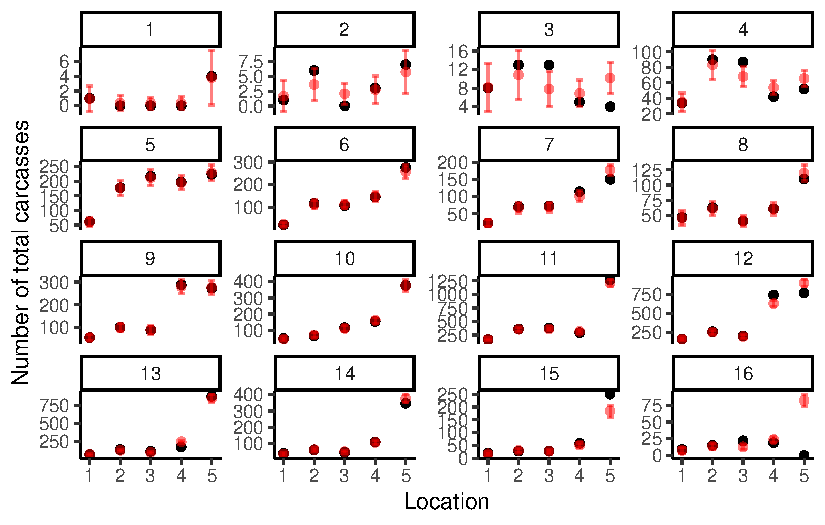
\includegraphics{KaleDoc_files/figure-pdf/unnamed-chunk-5-1.pdf}

}

\end{figure}

\hypertarget{carcass-tagging-rate-c_ts-times-psi_ts}{%
\paragraph{\texorpdfstring{Carcass tagging rate,
\(C_{t,s} \times \psi_{t,s}\)}{Carcass tagging rate, C\_\{t,s\} \textbackslash times \textbackslash psi\_\{t,s\}}}\label{carcass-tagging-rate-c_ts-times-psi_ts}}

\begin{Shaded}
\begin{Highlighting}[]
\NormalTok{E }\OtherTok{\textless{}{-}}\NormalTok{ reshape2}\SpecialCharTok{::}\FunctionTok{melt}\NormalTok{(sd.est}\SpecialCharTok{$}\NormalTok{E\_TaggedCarcasses\_t)}
\NormalTok{E}\SpecialCharTok{$}\NormalTok{sd }\OtherTok{\textless{}{-}}\NormalTok{ reshape2}\SpecialCharTok{::}\FunctionTok{melt}\NormalTok{(sd.sd}\SpecialCharTok{$}\NormalTok{E\_TaggedCarcasses\_t)}\SpecialCharTok{$}\NormalTok{value}
\NormalTok{E}\SpecialCharTok{$}\NormalTok{obs }\OtherTok{\textless{}{-}}\NormalTok{ reshape2}\SpecialCharTok{::}\FunctionTok{melt}\NormalTok{(rep}\SpecialCharTok{$}\NormalTok{TaggedCarcasses\_t)}\SpecialCharTok{$}\NormalTok{value}
\NormalTok{E }\SpecialCharTok{\%\textgreater{}\%} \FunctionTok{filter}\NormalTok{(Var1 }\SpecialCharTok{!=} \DecValTok{6}\NormalTok{) }\SpecialCharTok{\%\textgreater{}\%}
  \FunctionTok{ggplot}\NormalTok{(}\FunctionTok{aes}\NormalTok{(}\AttributeTok{x =}\NormalTok{ Var1, }\AttributeTok{y =}\NormalTok{ obs)) }\SpecialCharTok{+}
  \FunctionTok{geom\_point}\NormalTok{() }\SpecialCharTok{+}
  \FunctionTok{geom\_point}\NormalTok{(}\FunctionTok{aes}\NormalTok{(}\AttributeTok{x =}\NormalTok{ Var1, }\AttributeTok{y =}\NormalTok{ value), }\AttributeTok{color =} \StringTok{"red"}\NormalTok{, }\AttributeTok{alpha =} \FloatTok{0.5}\NormalTok{) }\SpecialCharTok{+}
  \FunctionTok{geom\_errorbar}\NormalTok{(}\FunctionTok{aes}\NormalTok{(}\AttributeTok{ymin =}\NormalTok{ value }\SpecialCharTok{{-}} \FloatTok{1.96} \SpecialCharTok{*}\NormalTok{ sd, }\AttributeTok{ymax =}\NormalTok{ value }\SpecialCharTok{+} \FloatTok{1.96} \SpecialCharTok{*}\NormalTok{ sd), }\AttributeTok{color =} \StringTok{"red"}\NormalTok{, }\AttributeTok{alpha =} \FloatTok{0.5}\NormalTok{, }\AttributeTok{width =} \FloatTok{0.2}\NormalTok{) }\SpecialCharTok{+}
  \FunctionTok{facet\_wrap}\NormalTok{(}\SpecialCharTok{\textasciitilde{}}\NormalTok{Var2, }\AttributeTok{ncol =} \DecValTok{4}\NormalTok{, }\AttributeTok{scales =} \StringTok{"free\_y"}\NormalTok{) }\SpecialCharTok{+}
  \FunctionTok{xlab}\NormalTok{(}\StringTok{"Location"}\NormalTok{) }\SpecialCharTok{+}
  \FunctionTok{ylab}\NormalTok{(}\StringTok{"Number of tagged carcasses"}\NormalTok{) }\SpecialCharTok{+}
  \FunctionTok{theme\_classic}\NormalTok{()}
\end{Highlighting}
\end{Shaded}

\begin{figure}[H]

{\centering 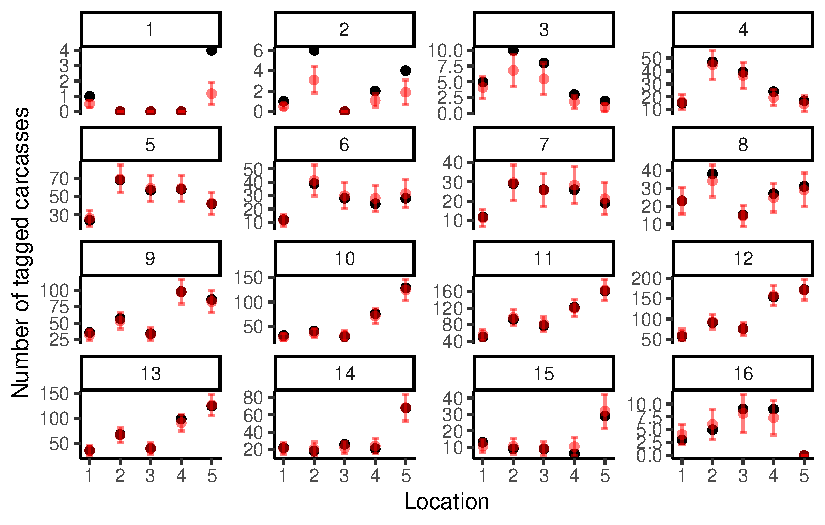
\includegraphics{KaleDoc_files/figure-pdf/unnamed-chunk-6-1.pdf}

}

\end{figure}

\hypertarget{mark-recapture-data-n_tmathrmt-times-phi-times-mathrmp}{%
\paragraph{\texorpdfstring{Mark-recapture data
\((N_{t,:})^\mathrm{T} \times \Phi \times \mathrm{p}\)}{Mark-recapture data (N\_\{t,:\})\^{}\textbackslash mathrm\{T\} \textbackslash times \textbackslash Phi \textbackslash times \textbackslash mathrm\{p\}}}\label{mark-recapture-data-n_tmathrmt-times-phi-times-mathrmp}}

These estimates represent the number of recaptured (y-axis) by recapture
location (x-axis) based on the tagging location (rows) and tagging
time-step (columns)

\begin{Shaded}
\begin{Highlighting}[]
\NormalTok{E }\OtherTok{\textless{}{-}}\NormalTok{ d }\SpecialCharTok{\%\textgreater{}\%}
  \FunctionTok{group\_by}\NormalTok{(t\_k, t\_l, tag) }\SpecialCharTok{\%\textgreater{}\%}
  \FunctionTok{mutate}\NormalTok{(}\AttributeTok{t\_k\_total =} \FunctionTok{sum}\NormalTok{(n))  }\SpecialCharTok{\%\textgreater{}\%}
  \FunctionTok{mutate}\NormalTok{(}\AttributeTok{obs =}\NormalTok{ n)}
\CommentTok{\# E$p \textless{}{-}  rep$probability\_of\_outcome}
\NormalTok{E}\SpecialCharTok{$}\NormalTok{pred }\OtherTok{\textless{}{-}}\NormalTok{ sd.est}\SpecialCharTok{$}\NormalTok{pred2}
\NormalTok{E}\SpecialCharTok{$}\NormalTok{sd }\OtherTok{\textless{}{-}}\NormalTok{ sd.sd}\SpecialCharTok{$}\NormalTok{pred2}

\NormalTok{E }\OtherTok{\textless{}{-}}\NormalTok{ E }\SpecialCharTok{\%\textgreater{}\%}
  \FunctionTok{filter}\NormalTok{(tag }\SpecialCharTok{==}\ConstantTok{TRUE}\NormalTok{) }\SpecialCharTok{\%\textgreater{}\%}
  \FunctionTok{group\_by}\NormalTok{(t\_k,t\_l,r\_l) }\SpecialCharTok{\%\textgreater{}\%}
  \FunctionTok{summarise}\NormalTok{(}\AttributeTok{obs =} \FunctionTok{sum}\NormalTok{(obs),}
            \AttributeTok{pred =} \FunctionTok{sum}\NormalTok{(}\FunctionTok{exp}\NormalTok{(pred)),}
            \AttributeTok{sd =} \FunctionTok{sum}\NormalTok{(sd))}
\end{Highlighting}
\end{Shaded}

\begin{verbatim}
`summarise()` has grouped output by 't_k', 't_l'. You can override using the
`.groups` argument.
\end{verbatim}

\begin{Shaded}
\begin{Highlighting}[]
\NormalTok{E }\SpecialCharTok{\%\textgreater{}\%}
  \FunctionTok{filter}\NormalTok{(t\_k}\SpecialCharTok{\textless{}=}\DecValTok{5}\NormalTok{) }\SpecialCharTok{\%\textgreater{}\%}
  \FunctionTok{mutate}\NormalTok{(}\AttributeTok{r\_l =} \FunctionTok{ifelse}\NormalTok{(}\FunctionTok{is.na}\NormalTok{(r\_l),}\DecValTok{6}\NormalTok{,r\_l)) }\SpecialCharTok{\%\textgreater{}\%}
  \FunctionTok{ggplot}\NormalTok{(}\FunctionTok{aes}\NormalTok{(}\AttributeTok{x =}\NormalTok{ r\_l, }\AttributeTok{y =}\NormalTok{ obs)) }\SpecialCharTok{+}
  \FunctionTok{geom\_point}\NormalTok{(}\AttributeTok{color =} \StringTok{"black"}\NormalTok{, }\AttributeTok{alpha =} \FloatTok{0.8}\NormalTok{) }\SpecialCharTok{+}
  \FunctionTok{geom\_point}\NormalTok{(}\FunctionTok{aes}\NormalTok{(}\AttributeTok{x =}\NormalTok{ r\_l, }\AttributeTok{y =}\NormalTok{ (pred)), }\AttributeTok{col =} \StringTok{"red"}\NormalTok{, }\AttributeTok{alpha =} \FloatTok{0.5}\NormalTok{) }\SpecialCharTok{+}
  \FunctionTok{geom\_errorbar}\NormalTok{(}\FunctionTok{aes}\NormalTok{(}\AttributeTok{ymin =} \FunctionTok{exp}\NormalTok{(}\FunctionTok{log}\NormalTok{(pred) }\SpecialCharTok{{-}} \FloatTok{1.96} \SpecialCharTok{*}\NormalTok{ sd), }\AttributeTok{ymax =} \FunctionTok{exp}\NormalTok{(}\FunctionTok{log}\NormalTok{(pred) }\SpecialCharTok{+} \FloatTok{1.96} \SpecialCharTok{*}\NormalTok{ sd)), }\AttributeTok{col =} \StringTok{"red"}\NormalTok{, }\AttributeTok{alpha =} \FloatTok{0.5}\NormalTok{, }\AttributeTok{width =} \FloatTok{0.5}\NormalTok{) }\SpecialCharTok{+}
  \FunctionTok{facet\_grid}\NormalTok{(t\_l}\SpecialCharTok{\textasciitilde{}}\NormalTok{t\_k, }\AttributeTok{scales =} \StringTok{"free\_y"}\NormalTok{) }\SpecialCharTok{+}
  \FunctionTok{xlab}\NormalTok{(}\StringTok{"Recapture location"}\NormalTok{) }\SpecialCharTok{+}
  \FunctionTok{theme\_bw}\NormalTok{() }\SpecialCharTok{+}
  \FunctionTok{theme}\NormalTok{(}
    \AttributeTok{panel.grid.major =} \FunctionTok{element\_blank}\NormalTok{(),  }\CommentTok{\# Remove major grid lines}
    \AttributeTok{panel.grid.minor =} \FunctionTok{element\_blank}\NormalTok{()   }\CommentTok{\# Remove minor grid lines}
\NormalTok{  )}
\end{Highlighting}
\end{Shaded}

\begin{figure}[H]

{\centering 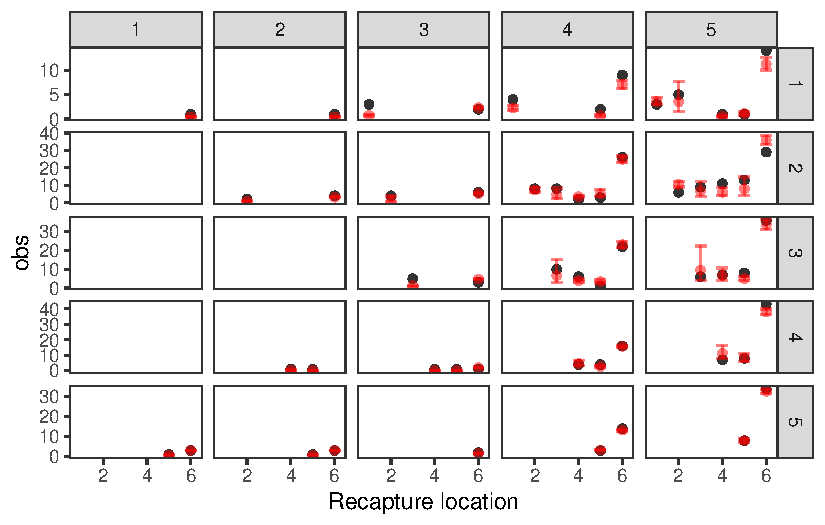
\includegraphics{KaleDoc_files/figure-pdf/unnamed-chunk-7-1.pdf}

}

\end{figure}

\begin{Shaded}
\begin{Highlighting}[]
\NormalTok{E }\SpecialCharTok{\%\textgreater{}\%}
  \FunctionTok{filter}\NormalTok{(t\_k}\SpecialCharTok{\textgreater{}}\DecValTok{5} \SpecialCharTok{\&}\NormalTok{ t\_k}\SpecialCharTok{\textless{}=}\DecValTok{10}\NormalTok{) }\SpecialCharTok{\%\textgreater{}\%}
  \FunctionTok{mutate}\NormalTok{(}\AttributeTok{r\_l =} \FunctionTok{ifelse}\NormalTok{(}\FunctionTok{is.na}\NormalTok{(r\_l),}\DecValTok{6}\NormalTok{,r\_l)) }\SpecialCharTok{\%\textgreater{}\%}
  \FunctionTok{ggplot}\NormalTok{(}\FunctionTok{aes}\NormalTok{(}\AttributeTok{x =}\NormalTok{ r\_l, }\AttributeTok{y =}\NormalTok{ obs)) }\SpecialCharTok{+}
  \FunctionTok{geom\_point}\NormalTok{(}\AttributeTok{color =} \StringTok{"black"}\NormalTok{, }\AttributeTok{alpha =} \FloatTok{0.8}\NormalTok{) }\SpecialCharTok{+}
  \FunctionTok{geom\_point}\NormalTok{(}\FunctionTok{aes}\NormalTok{(}\AttributeTok{x =}\NormalTok{ r\_l, }\AttributeTok{y =}\NormalTok{ (pred)), }\AttributeTok{col =} \StringTok{"red"}\NormalTok{, }\AttributeTok{alpha =} \FloatTok{0.5}\NormalTok{) }\SpecialCharTok{+}
  \FunctionTok{geom\_errorbar}\NormalTok{(}\FunctionTok{aes}\NormalTok{(}\AttributeTok{ymin =} \FunctionTok{exp}\NormalTok{(}\FunctionTok{log}\NormalTok{(pred) }\SpecialCharTok{{-}} \FloatTok{1.96} \SpecialCharTok{*}\NormalTok{ sd), }\AttributeTok{ymax =} \FunctionTok{exp}\NormalTok{(}\FunctionTok{log}\NormalTok{(pred) }\SpecialCharTok{+} \FloatTok{1.96} \SpecialCharTok{*}\NormalTok{ sd)), }\AttributeTok{col =} \StringTok{"red"}\NormalTok{, }\AttributeTok{alpha =} \FloatTok{0.5}\NormalTok{, }\AttributeTok{width =} \FloatTok{0.5}\NormalTok{) }\SpecialCharTok{+}
\FunctionTok{facet\_grid}\NormalTok{(t\_l}\SpecialCharTok{\textasciitilde{}}\NormalTok{t\_k, }\AttributeTok{scales =} \StringTok{"free\_y"}\NormalTok{) }\SpecialCharTok{+}
    \FunctionTok{xlab}\NormalTok{(}\StringTok{"Recapture location"}\NormalTok{) }\SpecialCharTok{+}
  \FunctionTok{theme\_bw}\NormalTok{() }\SpecialCharTok{+}
  \FunctionTok{theme}\NormalTok{(}
    \AttributeTok{panel.grid.major =} \FunctionTok{element\_blank}\NormalTok{(),  }\CommentTok{\# Remove major grid lines}
    \AttributeTok{panel.grid.minor =} \FunctionTok{element\_blank}\NormalTok{()   }\CommentTok{\# Remove minor grid lines}
\NormalTok{  )}
\end{Highlighting}
\end{Shaded}

\begin{figure}[H]

{\centering 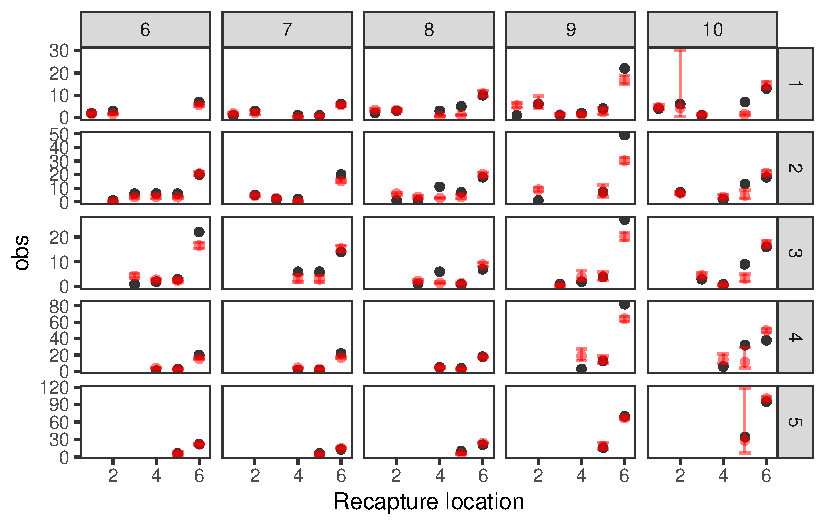
\includegraphics{KaleDoc_files/figure-pdf/unnamed-chunk-8-1.pdf}

}

\end{figure}

\begin{Shaded}
\begin{Highlighting}[]
\NormalTok{E }\SpecialCharTok{\%\textgreater{}\%}
  \FunctionTok{filter}\NormalTok{(t\_k}\SpecialCharTok{\textgreater{}}\DecValTok{11} \SpecialCharTok{\&}\NormalTok{ t\_k}\SpecialCharTok{\textless{}=}\DecValTok{16}\NormalTok{) }\SpecialCharTok{\%\textgreater{}\%}
  \FunctionTok{mutate}\NormalTok{(}\AttributeTok{r\_l =} \FunctionTok{ifelse}\NormalTok{(}\FunctionTok{is.na}\NormalTok{(r\_l),}\DecValTok{6}\NormalTok{,r\_l)) }\SpecialCharTok{\%\textgreater{}\%}
  \FunctionTok{ggplot}\NormalTok{(}\FunctionTok{aes}\NormalTok{(}\AttributeTok{x =}\NormalTok{ r\_l, }\AttributeTok{y =}\NormalTok{ obs)) }\SpecialCharTok{+}
  \FunctionTok{geom\_point}\NormalTok{(}\AttributeTok{color =} \StringTok{"black"}\NormalTok{, }\AttributeTok{alpha =} \FloatTok{0.8}\NormalTok{) }\SpecialCharTok{+}
  \FunctionTok{geom\_point}\NormalTok{(}\FunctionTok{aes}\NormalTok{(}\AttributeTok{x =}\NormalTok{ r\_l, }\AttributeTok{y =}\NormalTok{ (pred)), }\AttributeTok{col =} \StringTok{"red"}\NormalTok{, }\AttributeTok{alpha =} \FloatTok{0.5}\NormalTok{) }\SpecialCharTok{+}
  \FunctionTok{geom\_errorbar}\NormalTok{(}\FunctionTok{aes}\NormalTok{(}\AttributeTok{ymin =} \FunctionTok{exp}\NormalTok{(}\FunctionTok{log}\NormalTok{(pred) }\SpecialCharTok{{-}} \FloatTok{1.96} \SpecialCharTok{*}\NormalTok{ sd), }\AttributeTok{ymax =} \FunctionTok{exp}\NormalTok{(}\FunctionTok{log}\NormalTok{(pred) }\SpecialCharTok{+} \FloatTok{1.96} \SpecialCharTok{*}\NormalTok{ sd)), }\AttributeTok{col =} \StringTok{"red"}\NormalTok{, }\AttributeTok{alpha =} \FloatTok{0.5}\NormalTok{, }\AttributeTok{width =} \FloatTok{0.5}\NormalTok{) }\SpecialCharTok{+}
\FunctionTok{facet\_grid}\NormalTok{(t\_l}\SpecialCharTok{\textasciitilde{}}\NormalTok{t\_k, }\AttributeTok{scales =} \StringTok{"free\_y"}\NormalTok{) }\SpecialCharTok{+}
    \FunctionTok{xlab}\NormalTok{(}\StringTok{"Recapture location"}\NormalTok{) }\SpecialCharTok{+}
  \FunctionTok{theme\_bw}\NormalTok{() }\SpecialCharTok{+}
  \FunctionTok{theme}\NormalTok{(}
    \AttributeTok{panel.grid.major =} \FunctionTok{element\_blank}\NormalTok{(),  }\CommentTok{\# Remove major grid lines}
    \AttributeTok{panel.grid.minor =} \FunctionTok{element\_blank}\NormalTok{()   }\CommentTok{\# Remove minor grid lines}
\NormalTok{  )}
\end{Highlighting}
\end{Shaded}

\begin{figure}[H]

{\centering 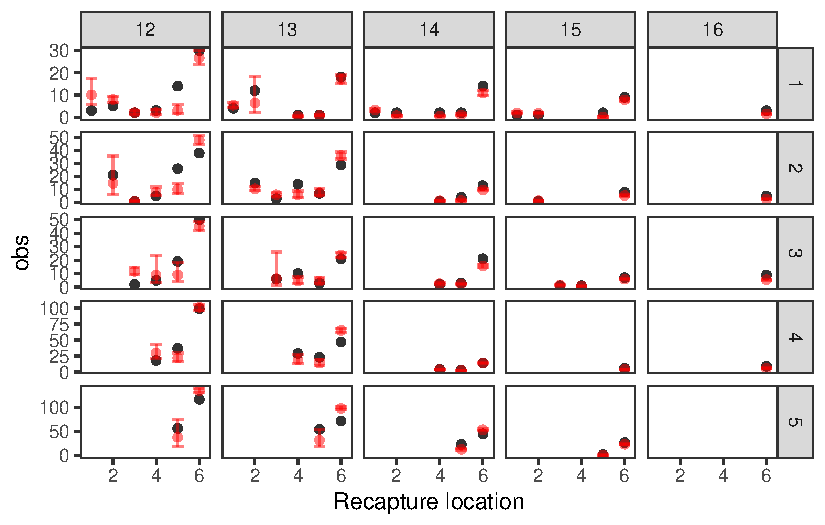
\includegraphics{KaleDoc_files/figure-pdf/unnamed-chunk-9-1.pdf}

}

\end{figure}

\hypertarget{derived-variables}{%
\subsubsection{Derived variables}\label{derived-variables}}

\hypertarget{total-births}{%
\paragraph{Total births}\label{total-births}}

\begin{Shaded}
\begin{Highlighting}[]
\NormalTok{E }\OtherTok{\textless{}{-}}\NormalTok{ reshape2}\SpecialCharTok{::}\FunctionTok{melt}\NormalTok{(sd.est}\SpecialCharTok{$}\NormalTok{B\_total)}
\NormalTok{E}\SpecialCharTok{$}\NormalTok{sd }\OtherTok{\textless{}{-}}\NormalTok{ reshape2}\SpecialCharTok{::}\FunctionTok{melt}\NormalTok{(sd.sd}\SpecialCharTok{$}\NormalTok{B\_total)}\SpecialCharTok{$}\NormalTok{value}
\NormalTok{x }\OtherTok{\textless{}{-}} \FunctionTok{rnorm}\NormalTok{(}\DecValTok{1000}\NormalTok{,sd.est}\SpecialCharTok{$}\NormalTok{B\_total,sd.sd}\SpecialCharTok{$}\NormalTok{B\_total)}
\FunctionTok{hist}\NormalTok{(}\FunctionTok{exp}\NormalTok{(x),}
     \AttributeTok{main =} \StringTok{""}\NormalTok{,}
     \AttributeTok{ylab =} \StringTok{""}\NormalTok{,}
     \AttributeTok{xlab =} \StringTok{"Total births"}\NormalTok{)}
\end{Highlighting}
\end{Shaded}

\begin{figure}[H]

{\centering 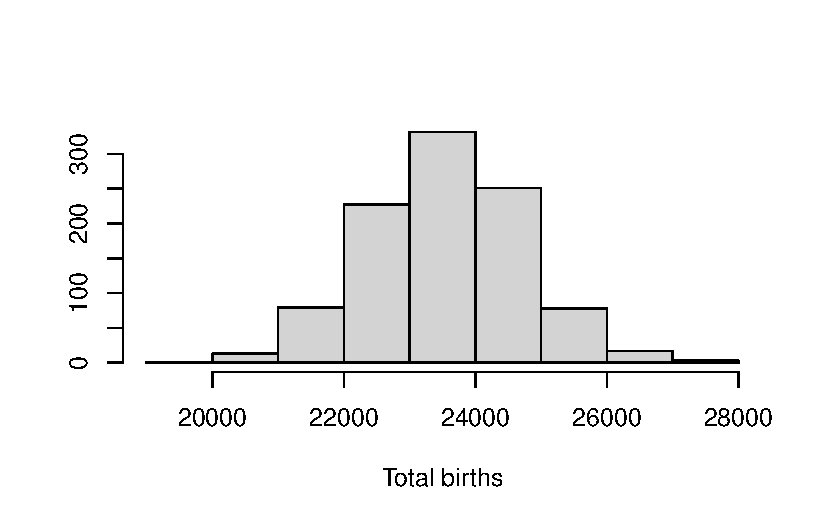
\includegraphics{KaleDoc_files/figure-pdf/unnamed-chunk-10-1.pdf}

}

\end{figure}

\begin{Shaded}
\begin{Highlighting}[]
\CommentTok{\#E \%\textgreater{}\% \#filter(Var1 != 6) \%\textgreater{}\%}
\CommentTok{\#  ggplot(aes(x = Var1, y = exp(value))) +}
\CommentTok{\#  geom\_col() +}
\CommentTok{\#  geom\_errorbar(aes(ymin = exp(value {-} 1.96 * sd), ymax = exp(value + 1.96 * sd))) +}
\CommentTok{\#  xlab("Location") +}
\CommentTok{\#  ylab("Total births") +}
\CommentTok{\#  theme\_classic()}
\end{Highlighting}
\end{Shaded}

\hypertarget{births-by-day-and-location}{%
\paragraph{Births by day and
location}\label{births-by-day-and-location}}

\begin{Shaded}
\begin{Highlighting}[]
\NormalTok{E }\OtherTok{\textless{}{-}}\NormalTok{ reshape2}\SpecialCharTok{::}\FunctionTok{melt}\NormalTok{(sd.est}\SpecialCharTok{$}\NormalTok{B\_ts)}
\NormalTok{E}\SpecialCharTok{$}\NormalTok{sd }\OtherTok{\textless{}{-}}\NormalTok{ reshape2}\SpecialCharTok{::}\FunctionTok{melt}\NormalTok{(sd.sd}\SpecialCharTok{$}\NormalTok{B\_ts)}\SpecialCharTok{$}\NormalTok{value}
\NormalTok{E }\SpecialCharTok{\%\textgreater{}\%} \CommentTok{\#filter(Var1 != 6) \%\textgreater{}\%}
  \FunctionTok{ggplot}\NormalTok{(}\FunctionTok{aes}\NormalTok{(}\AttributeTok{x =}\NormalTok{ Var1, }\AttributeTok{y =} \FunctionTok{exp}\NormalTok{(value))) }\SpecialCharTok{+}
  \FunctionTok{geom\_col}\NormalTok{() }\SpecialCharTok{+}
  \FunctionTok{geom\_errorbar}\NormalTok{(}\FunctionTok{aes}\NormalTok{(}\AttributeTok{ymin =} \FunctionTok{exp}\NormalTok{(value }\SpecialCharTok{{-}} \FloatTok{1.96} \SpecialCharTok{*}\NormalTok{ sd), }\AttributeTok{ymax =} \FunctionTok{exp}\NormalTok{(value }\SpecialCharTok{+} \FloatTok{1.96} \SpecialCharTok{*}\NormalTok{ sd))) }\SpecialCharTok{+}
  \FunctionTok{facet\_wrap}\NormalTok{(}\SpecialCharTok{\textasciitilde{}}\NormalTok{Var2, }\AttributeTok{ncol =} \DecValTok{4}\NormalTok{, }\AttributeTok{scales =} \StringTok{"free\_y"}\NormalTok{) }\SpecialCharTok{+}
  \FunctionTok{xlab}\NormalTok{(}\StringTok{"Location"}\NormalTok{) }\SpecialCharTok{+}
  \FunctionTok{ylab}\NormalTok{(}\StringTok{"Births"}\NormalTok{) }\SpecialCharTok{+}
  \FunctionTok{theme\_classic}\NormalTok{()}
\end{Highlighting}
\end{Shaded}

\begin{figure}[H]

{\centering 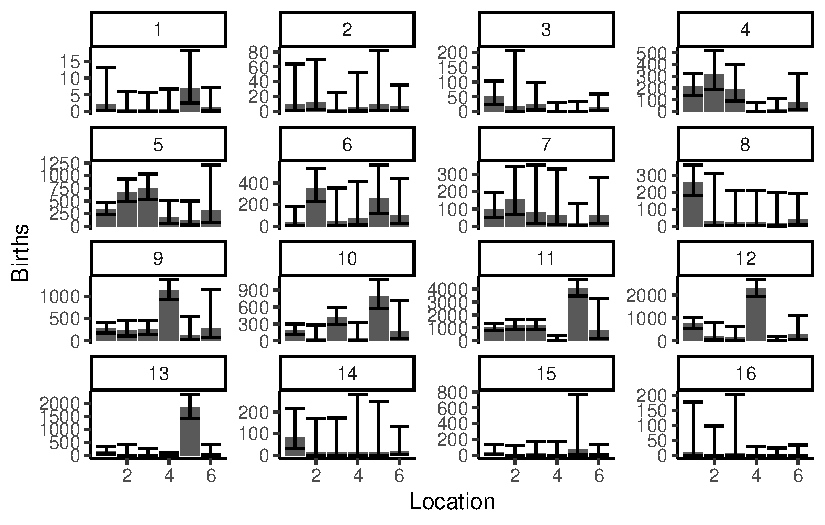
\includegraphics{KaleDoc_files/figure-pdf/unnamed-chunk-11-1.pdf}

}

\end{figure}

\hypertarget{total-carcasses}{%
\paragraph{Total carcasses}\label{total-carcasses}}

\hypertarget{parameters}{%
\subsubsection{Parameters}\label{parameters}}

\hypertarget{transition-matrix-psi}{%
\paragraph{\texorpdfstring{Transition matrix
\(\Psi\)}{Transition matrix \textbackslash Psi}}\label{transition-matrix-psi}}

\begin{Shaded}
\begin{Highlighting}[]
\NormalTok{p.mat }\OtherTok{\textless{}{-}}\NormalTok{ corrplot}\SpecialCharTok{::}\FunctionTok{cor.mtest}\NormalTok{(rep}\SpecialCharTok{$}\NormalTok{surv)}
\NormalTok{M }\OtherTok{\textless{}{-}}\NormalTok{ rep}\SpecialCharTok{$}\NormalTok{surv}
\CommentTok{\# M[6,6] \textless{}{-} NA}
\FunctionTok{colnames}\NormalTok{(M) }\OtherTok{\textless{}{-}} \FunctionTok{c}\NormalTok{(}\FunctionTok{paste}\NormalTok{(}\StringTok{"NLL"}\NormalTok{, }\DecValTok{1}\SpecialCharTok{:}\DecValTok{5}\NormalTok{),}\StringTok{"\textquotesingle{}Death\textquotesingle{}"}\NormalTok{)}
\FunctionTok{rownames}\NormalTok{(M) }\OtherTok{\textless{}{-}} \FunctionTok{c}\NormalTok{(}\FunctionTok{paste}\NormalTok{(}\StringTok{"NLL"}\NormalTok{, }\DecValTok{1}\SpecialCharTok{:}\DecValTok{5}\NormalTok{),}\StringTok{"\textquotesingle{}Death\textquotesingle{}"}\NormalTok{)}

\NormalTok{corrplot}\SpecialCharTok{::}\FunctionTok{corrplot}\NormalTok{(}
\NormalTok{  M, }
  
  \AttributeTok{method =} \StringTok{"color"}\NormalTok{,       }\CommentTok{\# or "color", "ellipse", etc.}
  \AttributeTok{type =} \StringTok{"upper"}\NormalTok{,          }\CommentTok{\# upper or lower triangle of correlation matrix}
  \AttributeTok{addCoef.col =} \StringTok{"black"}\NormalTok{,   }\CommentTok{\# color of correlation coefficients}
  \AttributeTok{tl.col =} \StringTok{"black"}\NormalTok{,        }\CommentTok{\# color of text labels (variable names)}
  \AttributeTok{tl.srt =} \DecValTok{45}\NormalTok{,}
  \AttributeTok{col.lim =} \FunctionTok{c}\NormalTok{(}\DecValTok{0}\NormalTok{,}\DecValTok{1}\NormalTok{)}
  \CommentTok{\# text label rotation}
\NormalTok{)}
\end{Highlighting}
\end{Shaded}

\begin{figure}[H]

{\centering 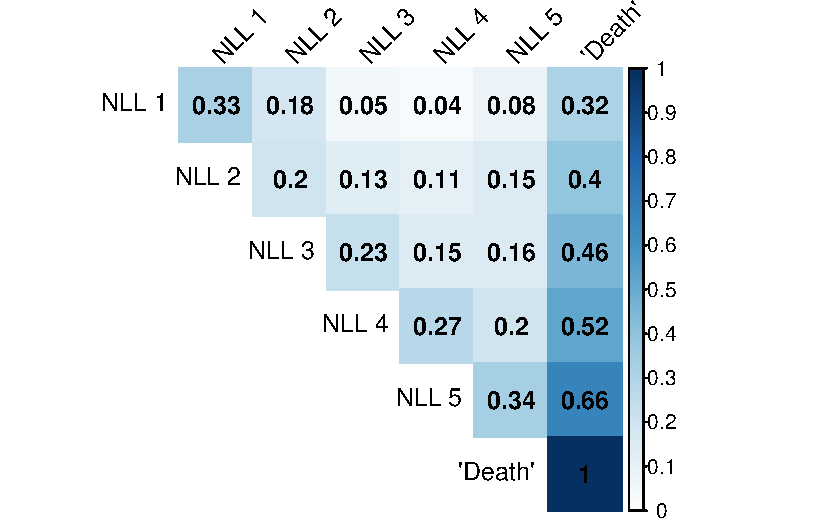
\includegraphics{KaleDoc_files/figure-pdf/unnamed-chunk-12-1.pdf}

}

\end{figure}

\hypertarget{detection-matrix-mathrmp}{%
\paragraph{\texorpdfstring{Detection matrix
\(\mathrm{p}\)}{Detection matrix \textbackslash mathrm\{p\}}}\label{detection-matrix-mathrmp}}

\begin{Shaded}
\begin{Highlighting}[]
\NormalTok{p.mat }\OtherTok{\textless{}{-}}\NormalTok{ corrplot}\SpecialCharTok{::}\FunctionTok{cor.mtest}\NormalTok{(rep}\SpecialCharTok{$}\NormalTok{p)}
\NormalTok{M }\OtherTok{\textless{}{-}}\NormalTok{ rep}\SpecialCharTok{$}\NormalTok{p}
\CommentTok{\# M[6,6] \textless{}{-} NA}
\FunctionTok{colnames}\NormalTok{(M) }\OtherTok{\textless{}{-}} \FunctionTok{c}\NormalTok{(}\FunctionTok{paste}\NormalTok{(}\StringTok{"NLL"}\NormalTok{, }\DecValTok{1}\SpecialCharTok{:}\DecValTok{5}\NormalTok{),}\StringTok{"\textquotesingle{}Non{-}detect\textquotesingle{}"}\NormalTok{)}
\FunctionTok{rownames}\NormalTok{(M) }\OtherTok{\textless{}{-}} \FunctionTok{c}\NormalTok{(}\FunctionTok{paste}\NormalTok{(}\StringTok{"NLL"}\NormalTok{, }\DecValTok{1}\SpecialCharTok{:}\DecValTok{5}\NormalTok{),}\StringTok{"\textquotesingle{}Non{-}detect\textquotesingle{}"}\NormalTok{)}

\NormalTok{corrplot}\SpecialCharTok{::}\FunctionTok{corrplot}\NormalTok{(}
\NormalTok{  M, }
  
  \AttributeTok{method =} \StringTok{"color"}\NormalTok{,       }\CommentTok{\# or "color", "ellipse", etc.}
  \AttributeTok{type =} \StringTok{"upper"}\NormalTok{,          }\CommentTok{\# upper or lower triangle of correlation matrix}
  \AttributeTok{addCoef.col =} \StringTok{"black"}\NormalTok{,   }\CommentTok{\# color of correlation coefficients}
  \AttributeTok{tl.col =} \StringTok{"black"}\NormalTok{,        }\CommentTok{\# color of text labels (variable names)}
  \AttributeTok{tl.srt =} \DecValTok{45}\NormalTok{,}
  \AttributeTok{col.lim =} \FunctionTok{c}\NormalTok{(}\DecValTok{0}\NormalTok{,}\DecValTok{1}\NormalTok{)}
  \CommentTok{\# text label rotation}
\NormalTok{)}
\end{Highlighting}
\end{Shaded}

\begin{figure}[H]

{\centering 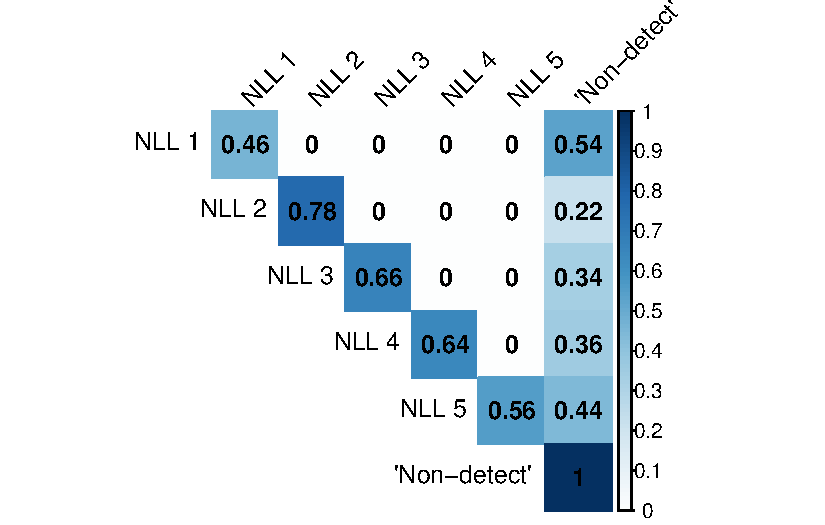
\includegraphics{KaleDoc_files/figure-pdf/unnamed-chunk-13-1.pdf}

}

\end{figure}

\hypertarget{tagging-rate}{%
\paragraph{Tagging rate}\label{tagging-rate}}

\begin{Shaded}
\begin{Highlighting}[]
\NormalTok{E }\OtherTok{\textless{}{-}}\NormalTok{ reshape2}\SpecialCharTok{::}\FunctionTok{melt}\NormalTok{(sd.est}\SpecialCharTok{$}\NormalTok{taggingRate)}
\NormalTok{E}\SpecialCharTok{$}\NormalTok{sd }\OtherTok{\textless{}{-}}\NormalTok{ reshape2}\SpecialCharTok{::}\FunctionTok{melt}\NormalTok{(sd.sd}\SpecialCharTok{$}\NormalTok{taggingRate)}\SpecialCharTok{$}\NormalTok{value}
\NormalTok{E }\SpecialCharTok{\%\textgreater{}\%} \CommentTok{\#filter(Var1 != 6) \%\textgreater{}\%}
  \FunctionTok{ggplot}\NormalTok{(}\FunctionTok{aes}\NormalTok{(}\AttributeTok{x =}\NormalTok{ Var2, }\AttributeTok{y =}\NormalTok{ (value))) }\SpecialCharTok{+}
  \FunctionTok{geom\_point}\NormalTok{() }\SpecialCharTok{+}
  \FunctionTok{geom\_errorbar}\NormalTok{(}\FunctionTok{aes}\NormalTok{(}\AttributeTok{ymin =}\NormalTok{ (value }\SpecialCharTok{{-}} \FloatTok{1.96} \SpecialCharTok{*}\NormalTok{ sd), }\AttributeTok{ymax =}\NormalTok{ (value }\SpecialCharTok{+} \FloatTok{1.96} \SpecialCharTok{*}\NormalTok{ sd))) }\SpecialCharTok{+}
  \FunctionTok{facet\_wrap}\NormalTok{(}\SpecialCharTok{\textasciitilde{}}\NormalTok{Var1, }\AttributeTok{ncol =} \DecValTok{2}\NormalTok{, }\AttributeTok{scales =} \StringTok{"free\_y"}\NormalTok{) }\SpecialCharTok{+}
  \FunctionTok{xlab}\NormalTok{(}\StringTok{"Location"}\NormalTok{) }\SpecialCharTok{+}
  \FunctionTok{ylab}\NormalTok{(}\StringTok{"Tagging rate"}\NormalTok{) }\SpecialCharTok{+}
  \FunctionTok{theme\_classic}\NormalTok{()}
\end{Highlighting}
\end{Shaded}

\begin{figure}[H]

{\centering 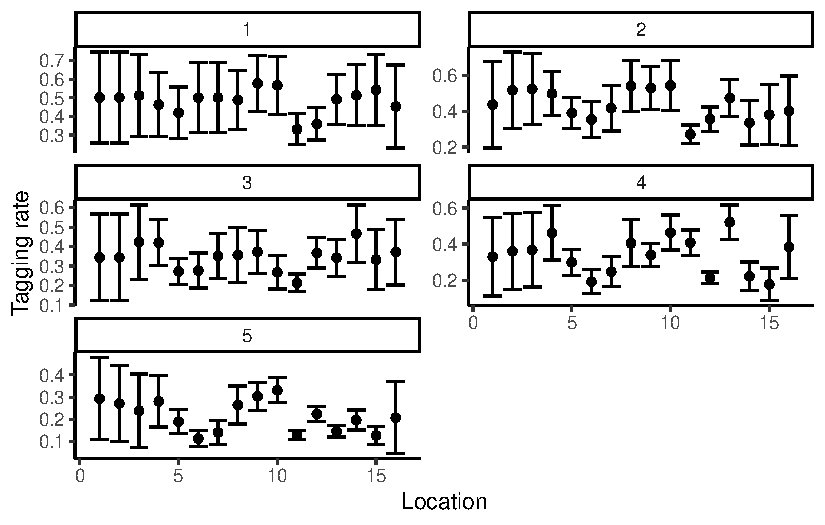
\includegraphics{KaleDoc_files/figure-pdf/unnamed-chunk-14-1.pdf}

}

\end{figure}



\end{document}
